
\section{Modelo de comportamiento del sistema}
En esta sección vamos a especificar cómo se comporta el sistema en forma de dos
elementos fundamentales.
\begin{itemize}
\item En primer lugar, los \textbf{diagramas de secuencia} mostrarán el flujo de
  eventos entre los actores que participan en la aplicación.
\item En segundo lugar, los \textbf{contratos de las operaciones} detallarán las
  condiciones y efectos que tendrán lugar al ejecutarse las operaciones en el
  sistema.
\end{itemize}

\begin{nota}
  No se han reflejado, por triviales, los escenarios alternativos en los que el
  usuario cierra la ventana, correspondientes a los flujos \textit{*a} definidos
  en la sección anterior.
\end{nota}

\subsection{Caso de uso: inicio del juego}

\subsubsection{Escenario principal}

\begin{figure}[h!]
  \centering
  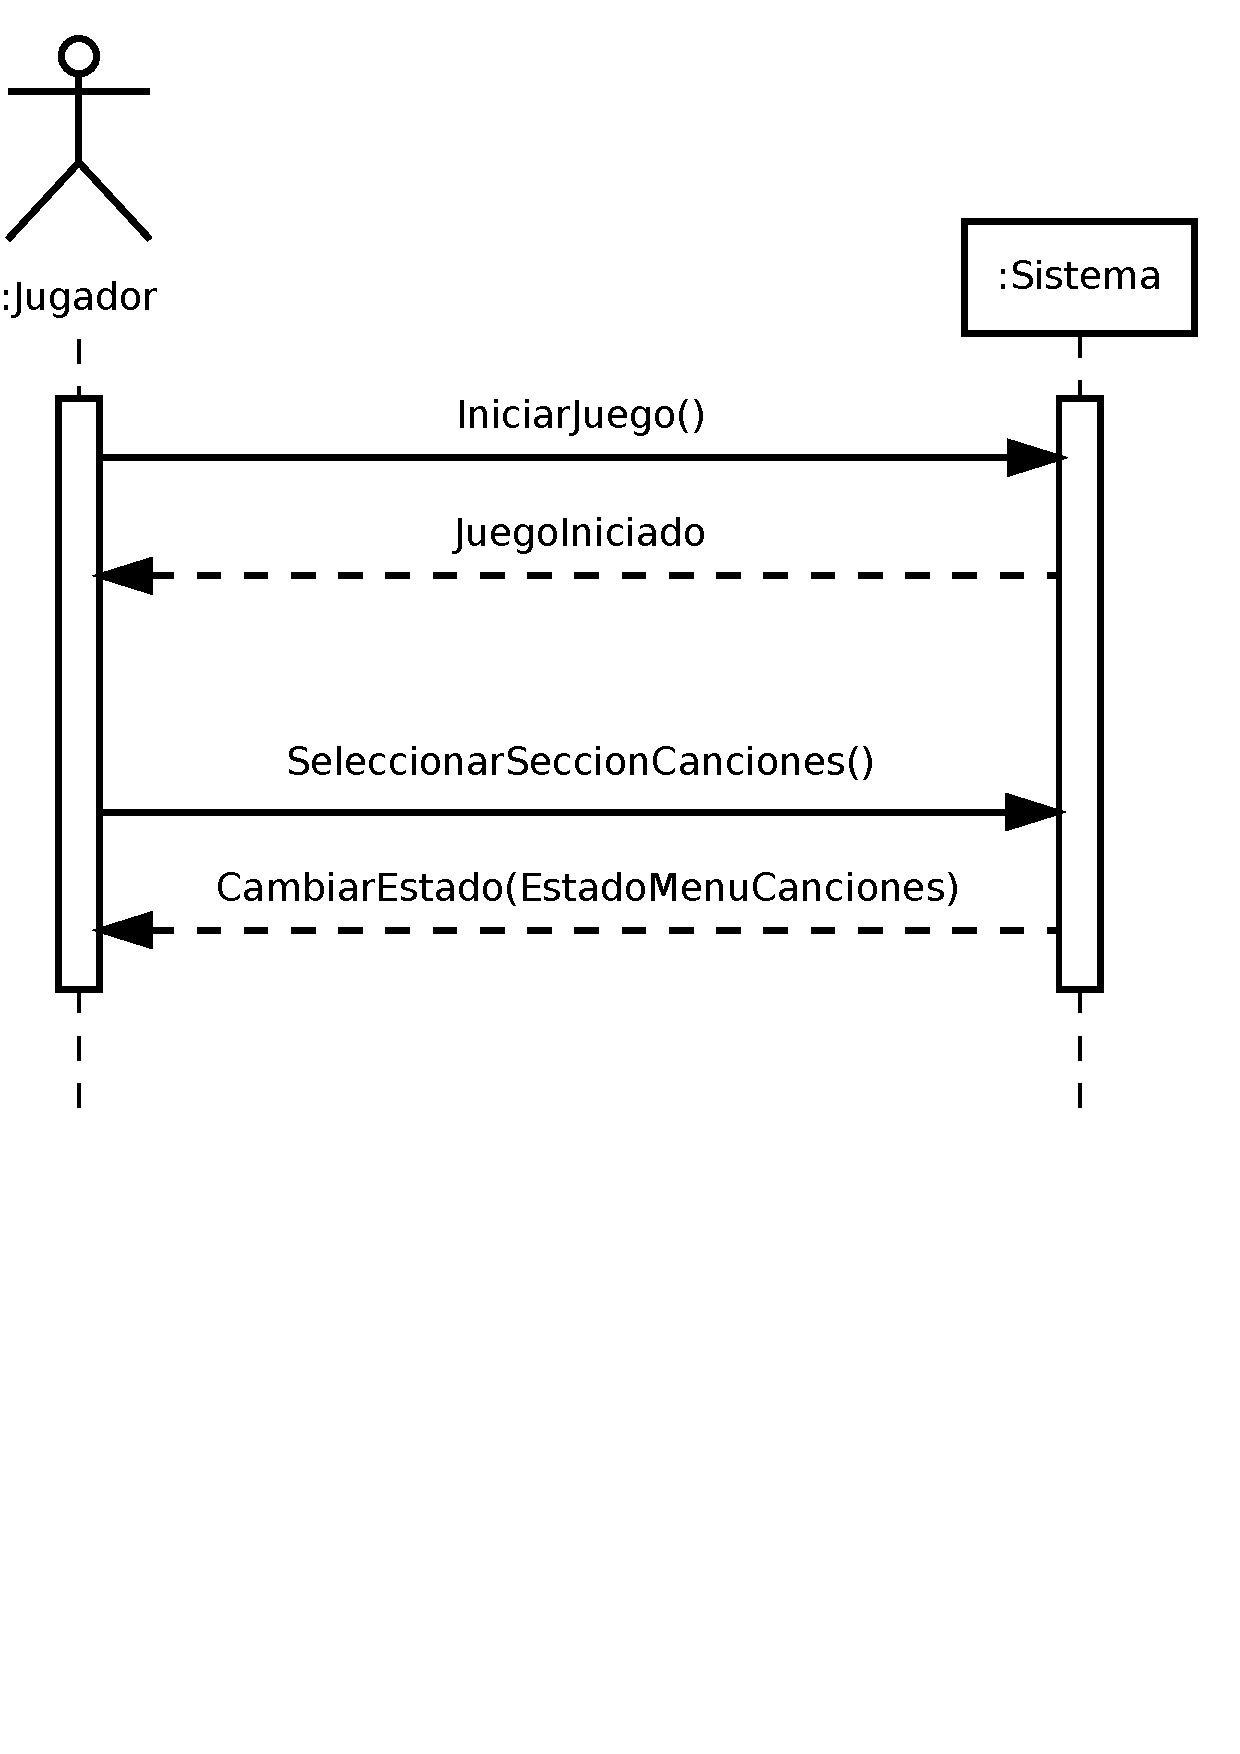
\includegraphics[trim=0cm 12cm 0cm 0cm, clip=true, width=0.5\textwidth]{4_analisis/diagsec_caso1_esc1}
  \caption{Diagrama de secuencia, incio del juego, escenario principal}
\end{figure}

\begin{description}
\item[Operación] IniciarJuego()
\item[Actores] \jugador\, \sistema\
\item[Responsabilidades] Cargar y lanzar la aplicación, mostrar los títulos de
  crédito y el menú principal.
\item[Precondiciones] Ninguna.
\item[Postcondiciones] $\quad$

  \begin{itemize}
  \item Se crea una instancia de la clase \textit{Juego}, que gestiona la
    creación y destrucción de los estados.
  \item Se crean y posteriormente destruyen dos estados
    \textit{EstadoImagenFija} para mostrar los títulos de crédito.
  \item Se crea y permanece un estado \textit{EstadoMenú}, que representa el
    menú principal de la aplicación.
  \end{itemize}

\end{description}

\begin{description}
\item[Operación] SeleccionarSeccionCanciones()
\item[Actores] \jugador\, \sistema\
\item[Responsabilidades] Esconder el menú principal y cargar el menú de
  selección de canciones.
\item[Precondiciones] $\quad$

  \begin{itemize}
  \item El estado actual es una instancia de \textit{EstadoMenú}.
  \end{itemize}

\item[Postcondiciones] Se destruye el estado \textit{EstadoMenú} y se carga
  \textit{EstadoMenúCanciones}.
\end{description}

\subsubsection{Escenario alternativo 4a}
\begin{figure}[h!]
  \centering
  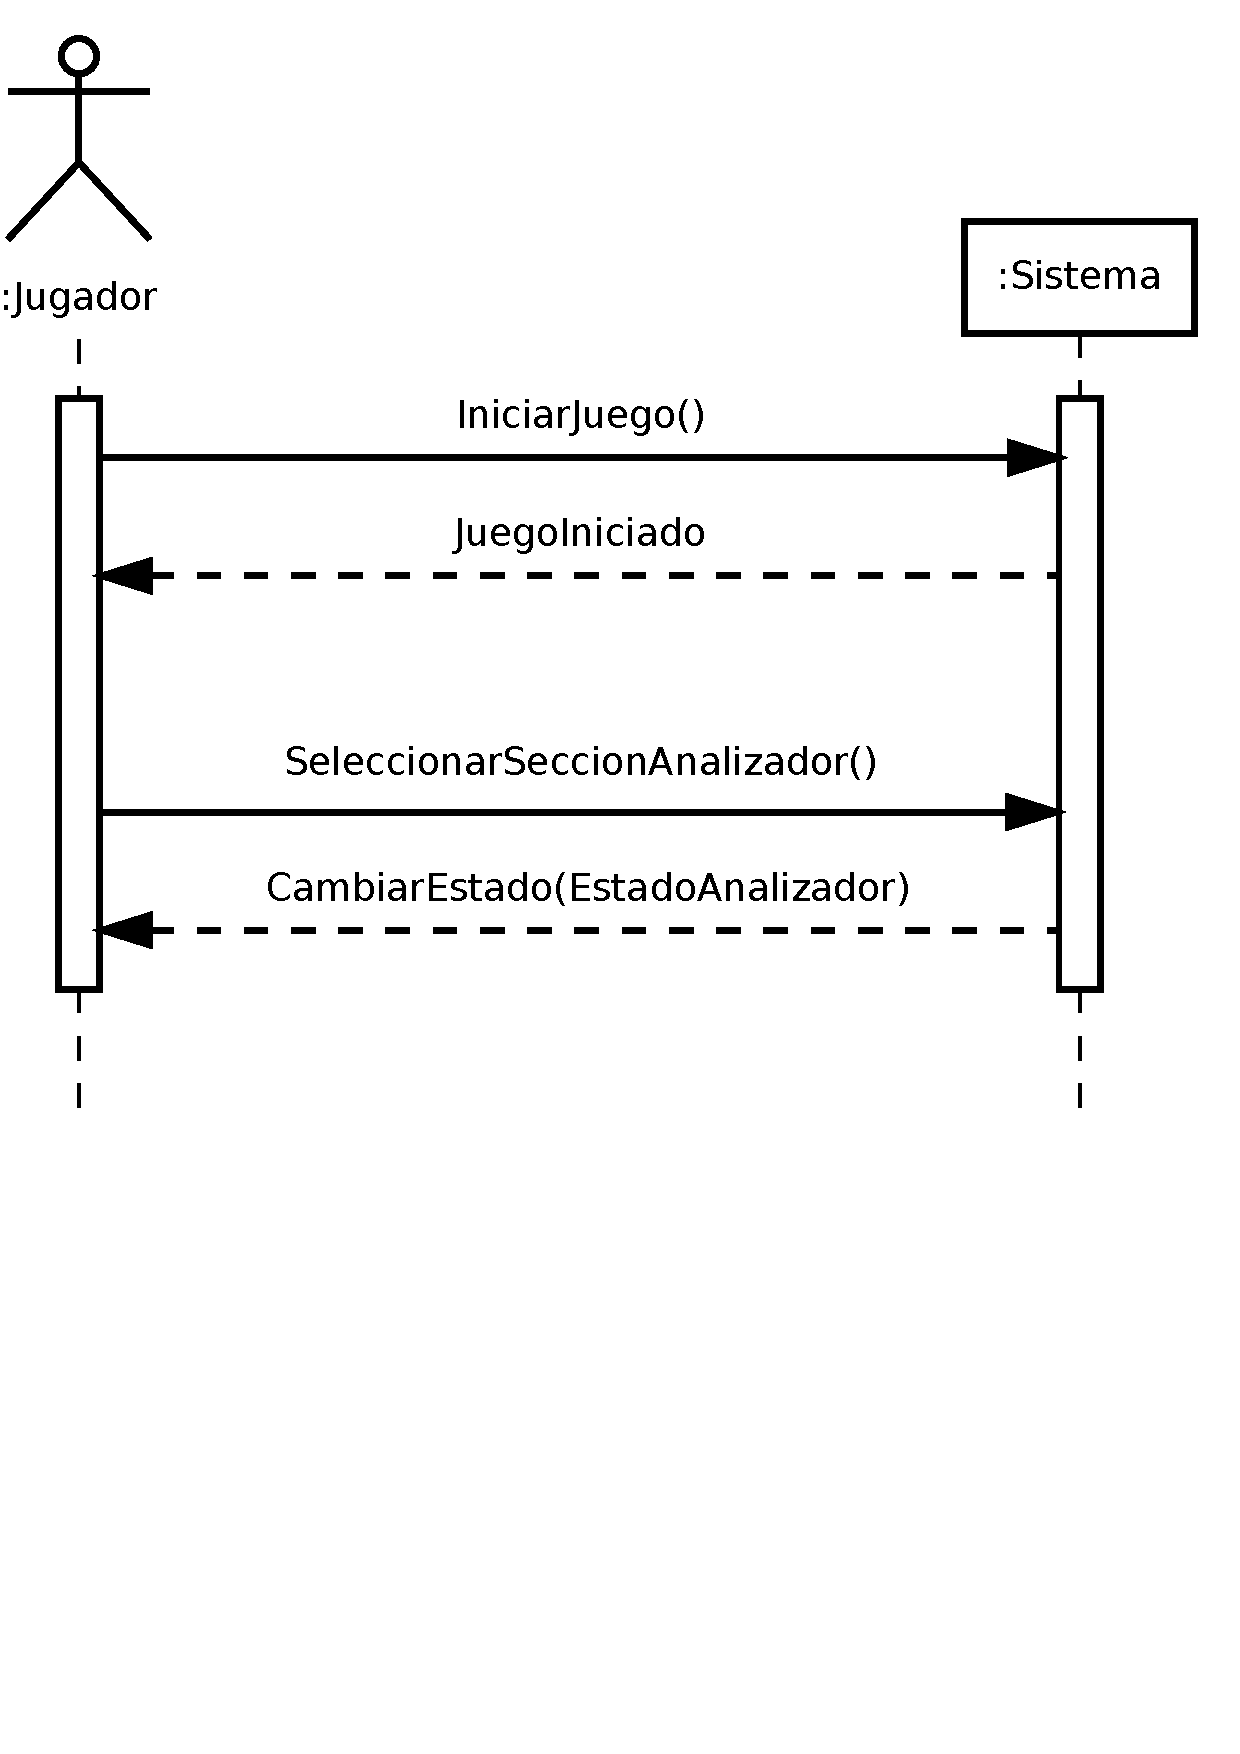
\includegraphics[trim=0cm 12cm 0cm 0cm, clip=true, width=0.5\textwidth]{4_analisis/diagsec_caso1_esc2}
  \caption{Diagrama de secuencia, incio del juego, escenario alternativo 4a}
\end{figure}

\begin{description}
\item[Operación] SeleccionarSeccionAnalizador()
\item[Actores] \jugador\, \sistema\
\item[Responsabilidades] Esconder el menú principal y cargar la sección de
  análisis de notas.
\item[Precondiciones] $\quad$
  \begin{itemize}
  \item El estado actual es una instancia de \textit{EstadoMenú}.
  \end{itemize}
\item[Postcondiciones] Se destruye el estado \textit{EstadoMenú} y se carga
  \textit{EstadoAnalizador}.
\end{description}

\subsubsection{Escenario alternativo 4b}
\begin{figure}[h!]
  \centering
  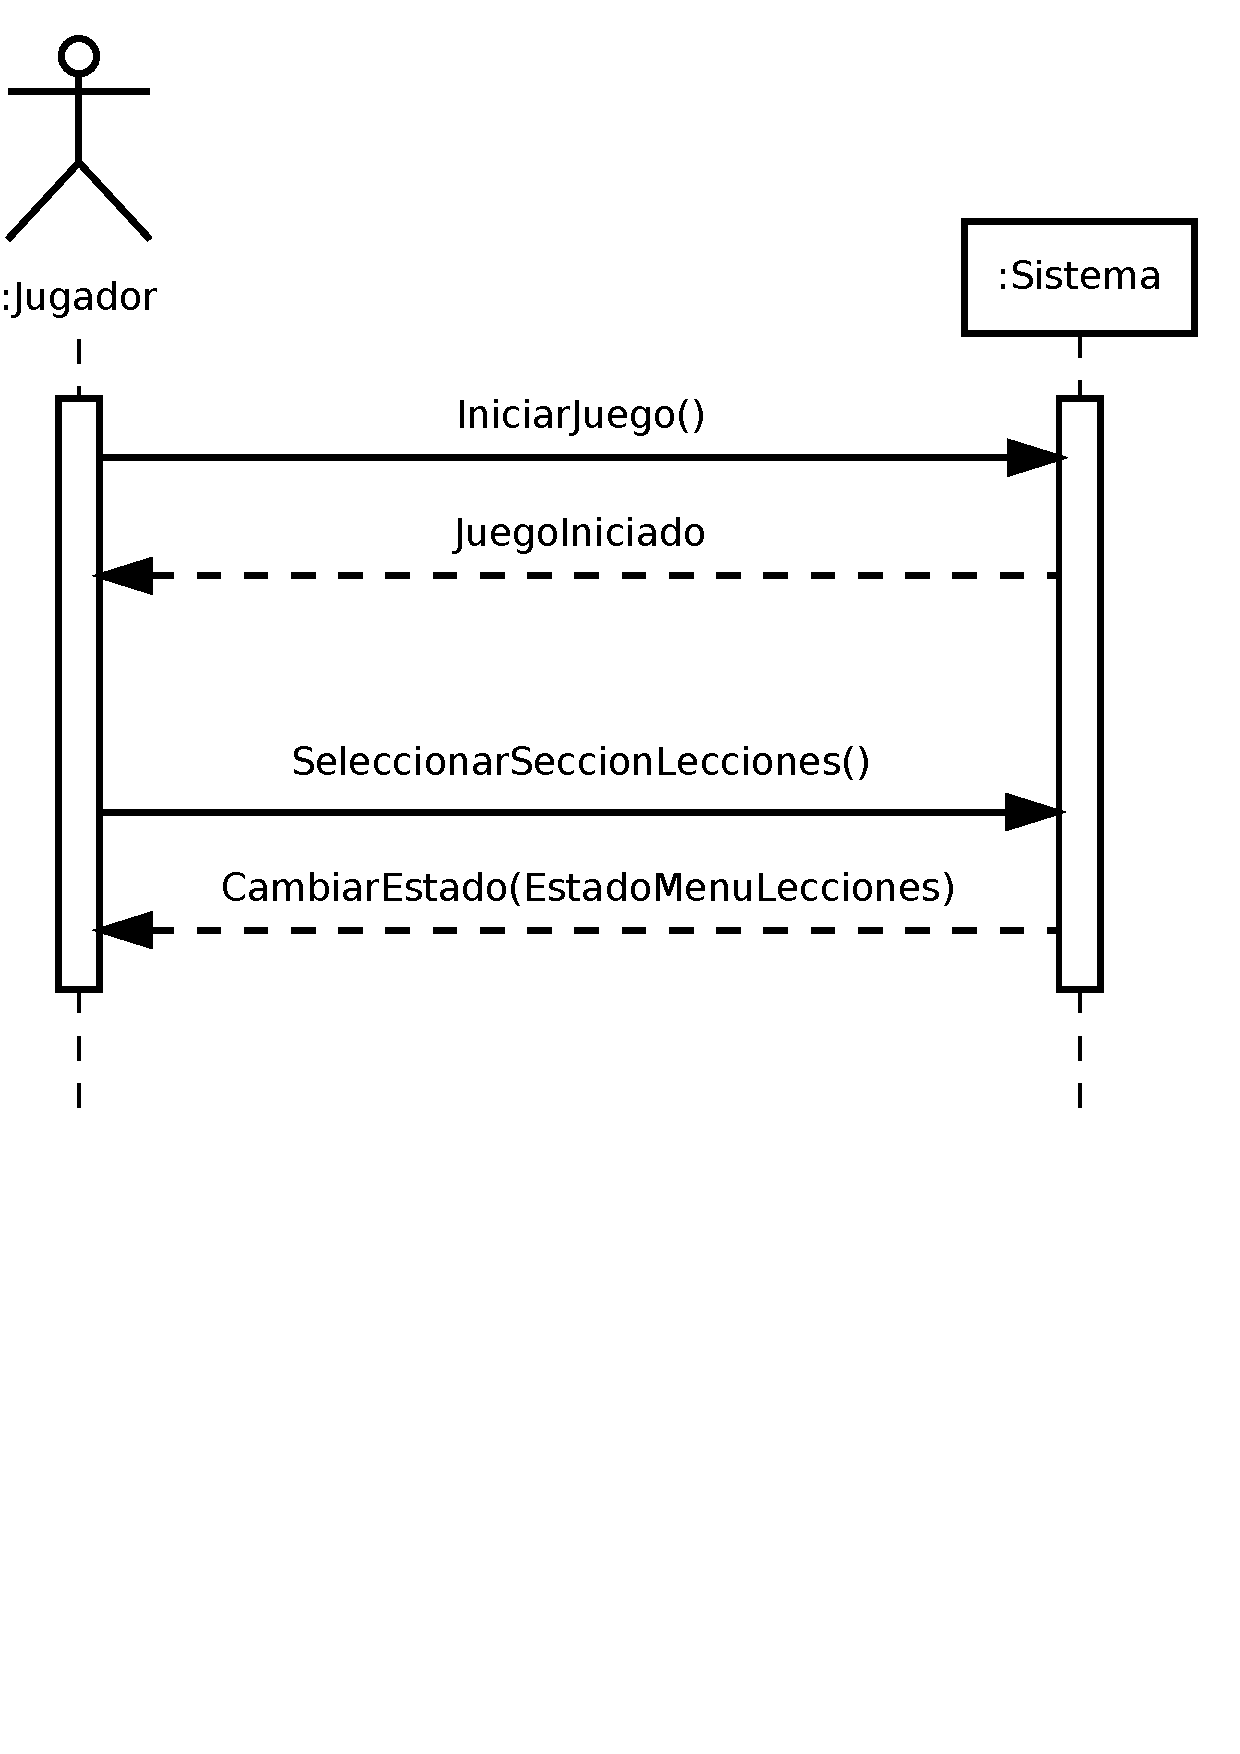
\includegraphics[trim=0cm 12cm 0cm 0cm, clip=true, width=0.5\textwidth]{4_analisis/diagsec_caso1_esc3}
  \caption{Diagrama de secuencia, incio del juego, escenario alternativo 4b}
\end{figure}

\begin{description}
\item[Operación] SeleccionarSeccionLecciones()
\item[Actores] \jugador\, \sistema\
\item[Responsabilidades] Esconder el menú principal y cargar la menú de
  selección de lecciones.
\item[Precondiciones] $\quad$
  \begin{itemize}
  \item El estado actual es una instancia de \textit{EstadoMenú}.
  \end{itemize}
\item[Postcondiciones] Se destruye el estado \textit{EstadoMenú} y se carga
  \textit{EstadoMenúLecciones}.
\end{description}

\subsubsection{Escenario alternativo 4c}
\begin{figure}[h!]
  \centering
  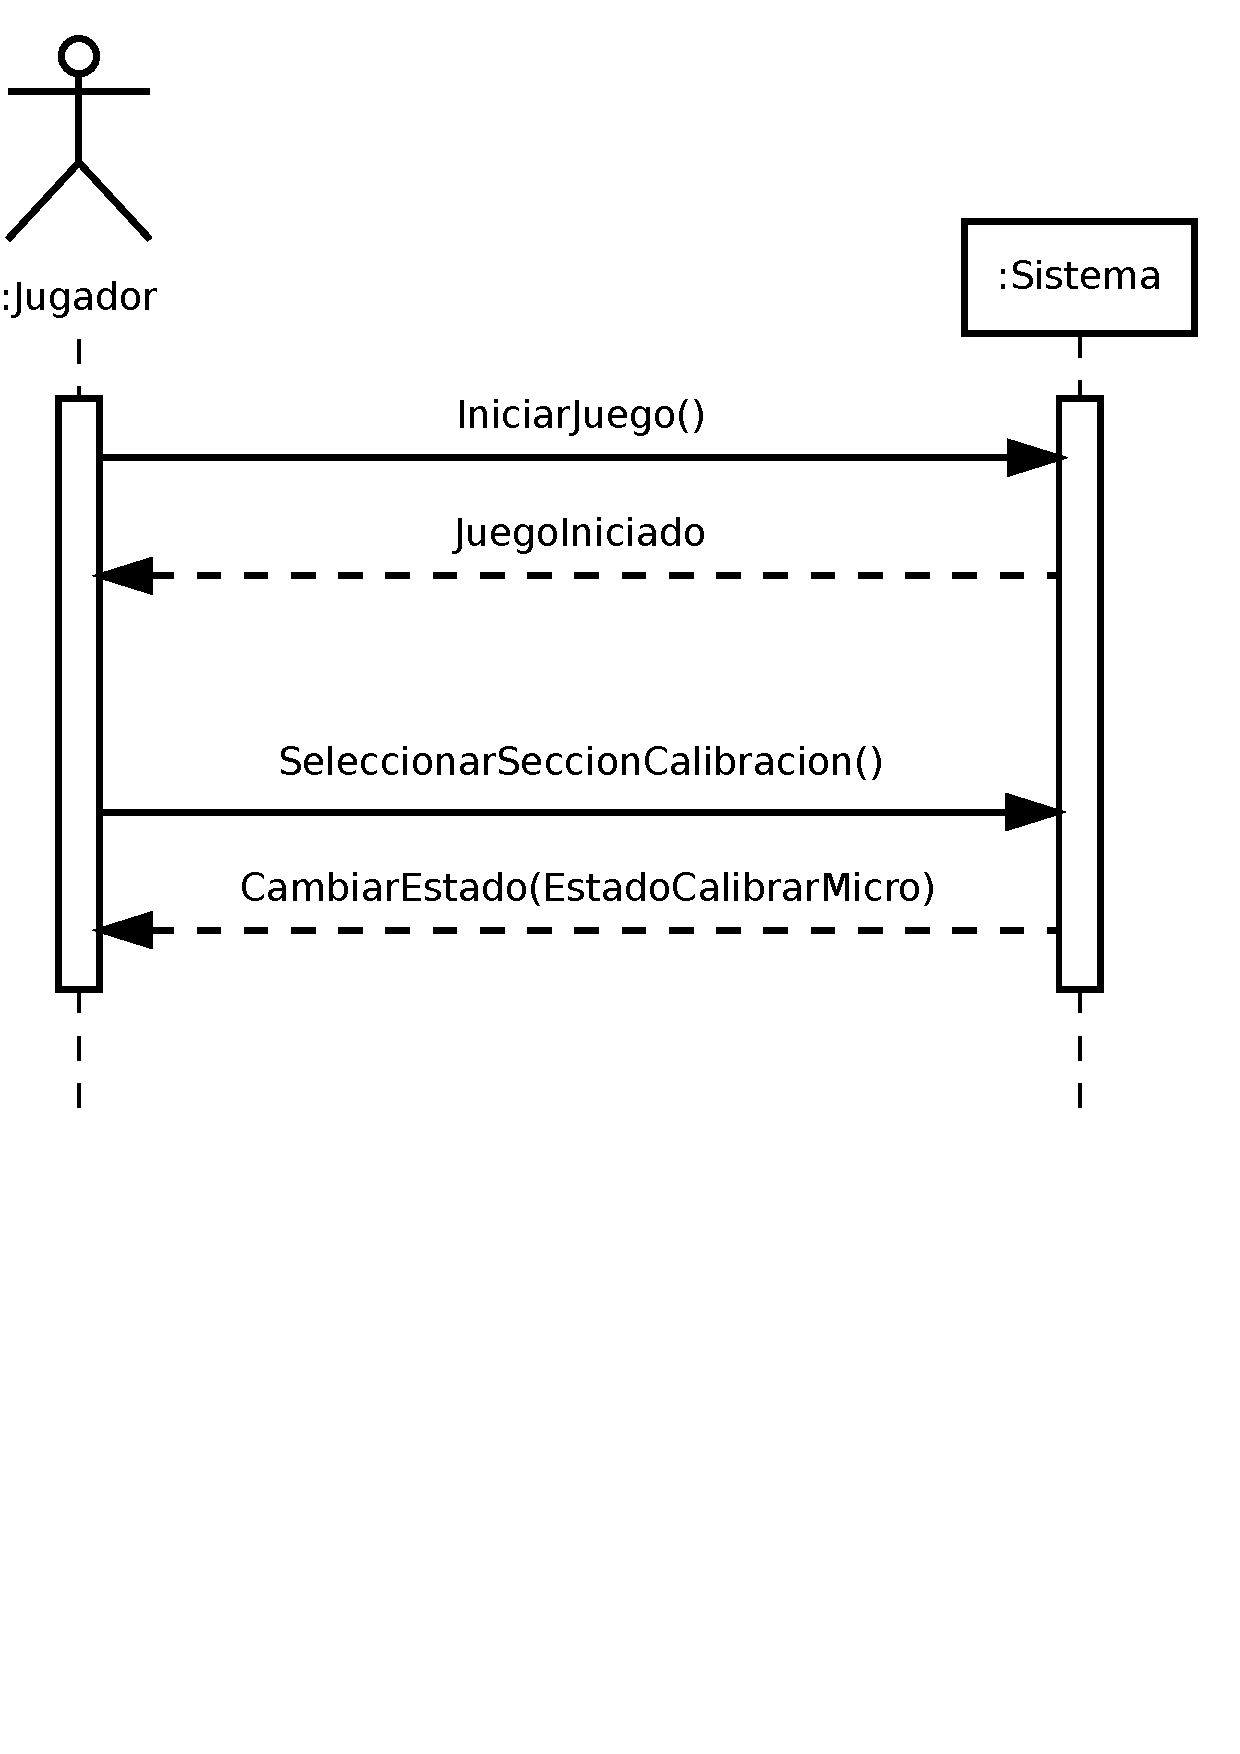
\includegraphics[trim=0cm 12cm 0cm 0cm, clip=true, width=0.5\textwidth]{4_analisis/diagsec_caso1_esc4}
  \caption{Diagrama de secuencia, incio del juego, escenario alternativo 4c}
\end{figure}

\begin{description}
\item[Operación] SeleccionarSeccionCalibracion()
\item[Actores] \jugador\, \sistema\
\item[Responsabilidades] Esconder el menú principal y cargar la sección de
  calibración de micrófono.
\item[Precondiciones] $\quad$
  \begin{itemize}
  \item El estado actual es una instancia de \textit{EstadoMenú}.
  \end{itemize}
\item[Postcondiciones] Se destruye el estado \textit{EstadoMenú} y se carga
  \textit{EstadoCalibrarMicro}.
\end{description}

\subsubsection{Escenario alternativo 4d}
\begin{figure}[h!]
  \centering
  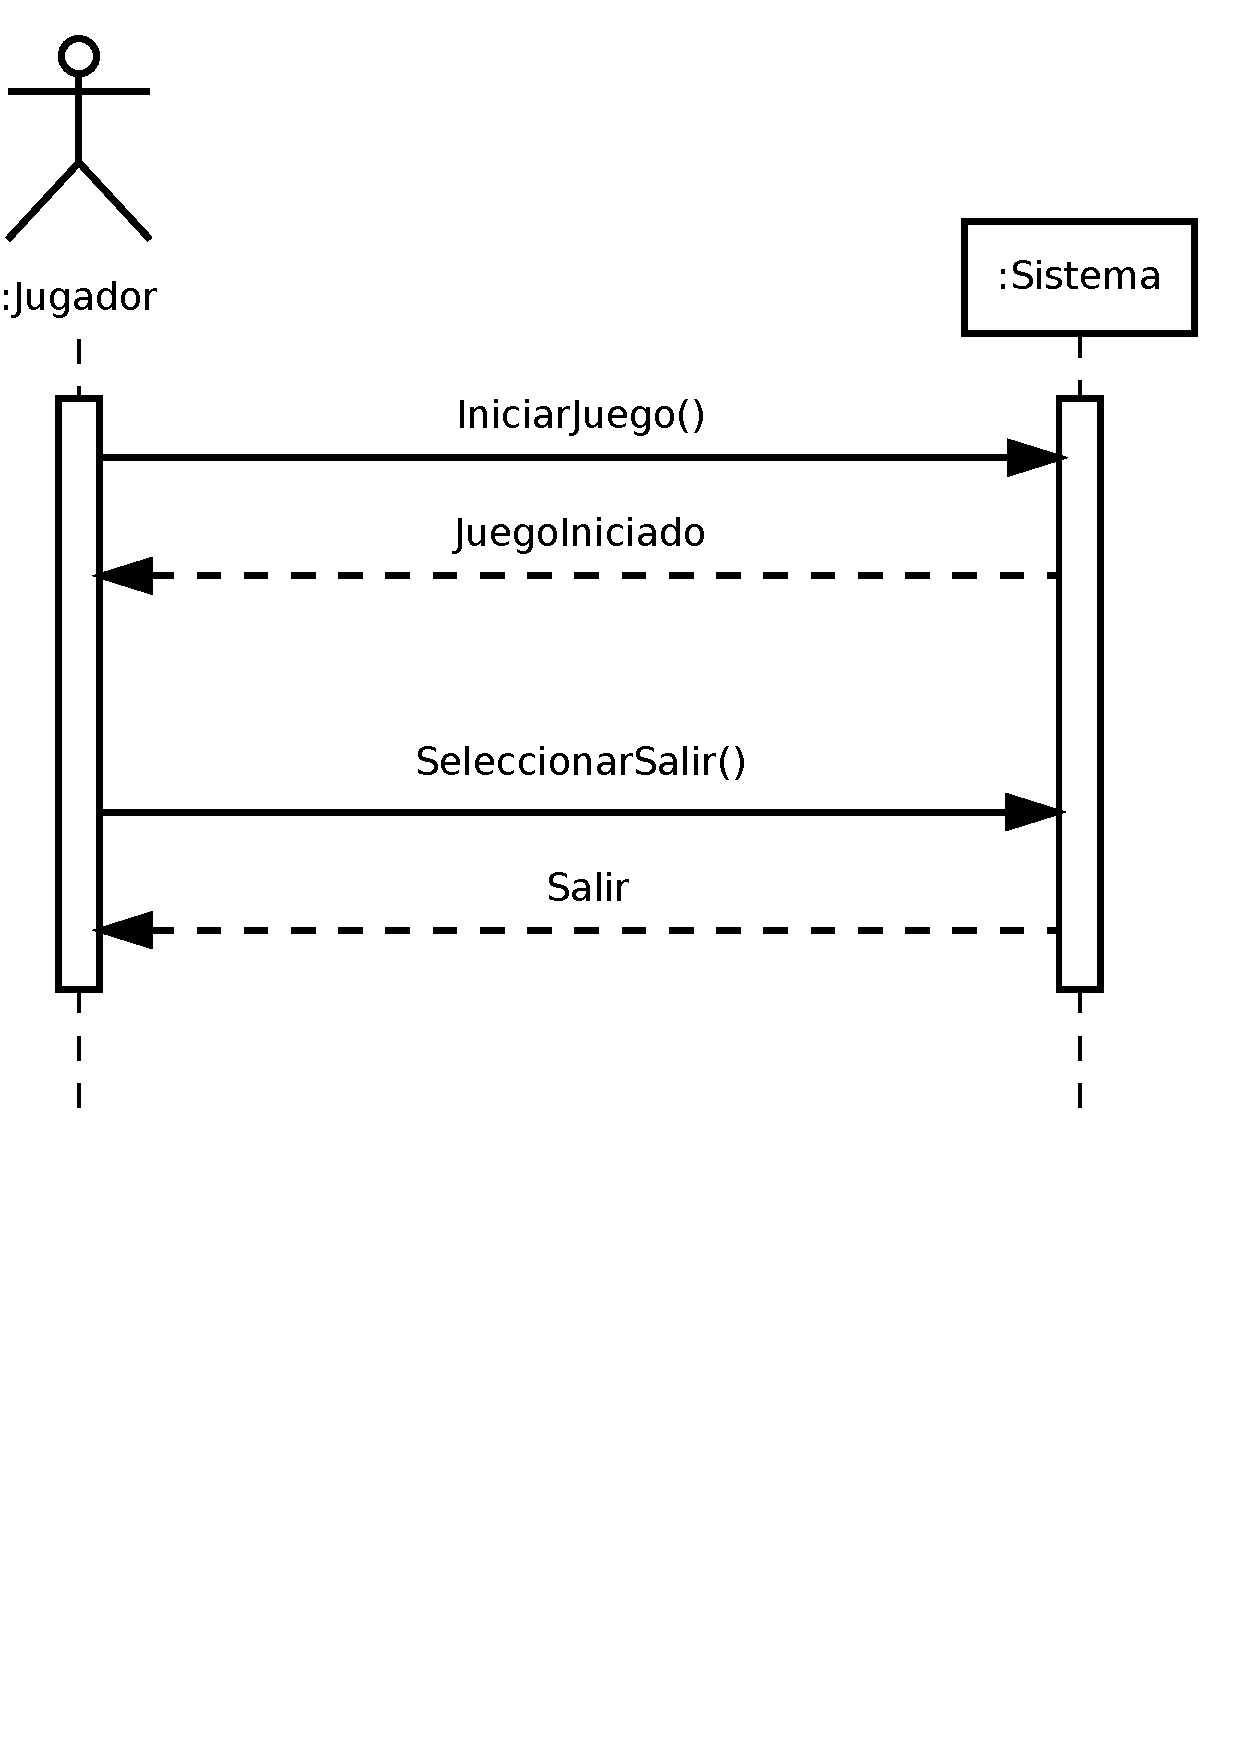
\includegraphics[trim=0cm 12cm 0cm 0cm, clip=true, width=0.5\textwidth]{4_analisis/diagsec_caso1_esc5}
  \caption{Diagrama de secuencia, incio del juego, escenario alternativo 4d}
\end{figure}

\begin{description}
\item[Operación] SeleccionarSalir()
\item[Actores] \jugador\, \sistema\
\item[Responsabilidades] Esconder el menú principal, descargar los recursos y
  cerrar la aplicación.
\item[Precondiciones] $\quad$
  \begin{itemize}
  \item El estado actual es una instancia de \textit{EstadoMenú}.
  \end{itemize}
\item[Postcondiciones] Se destruye el estado \textit{EstadoMenú}, se destruye la
  instancia de la clase \textit{Juego} y termina la ejecución de la aplicación.
\end{description}

\subsection{Selección de canción}

\subsubsection{Escenario principal}
\begin{figure}[h!]
  \centering
  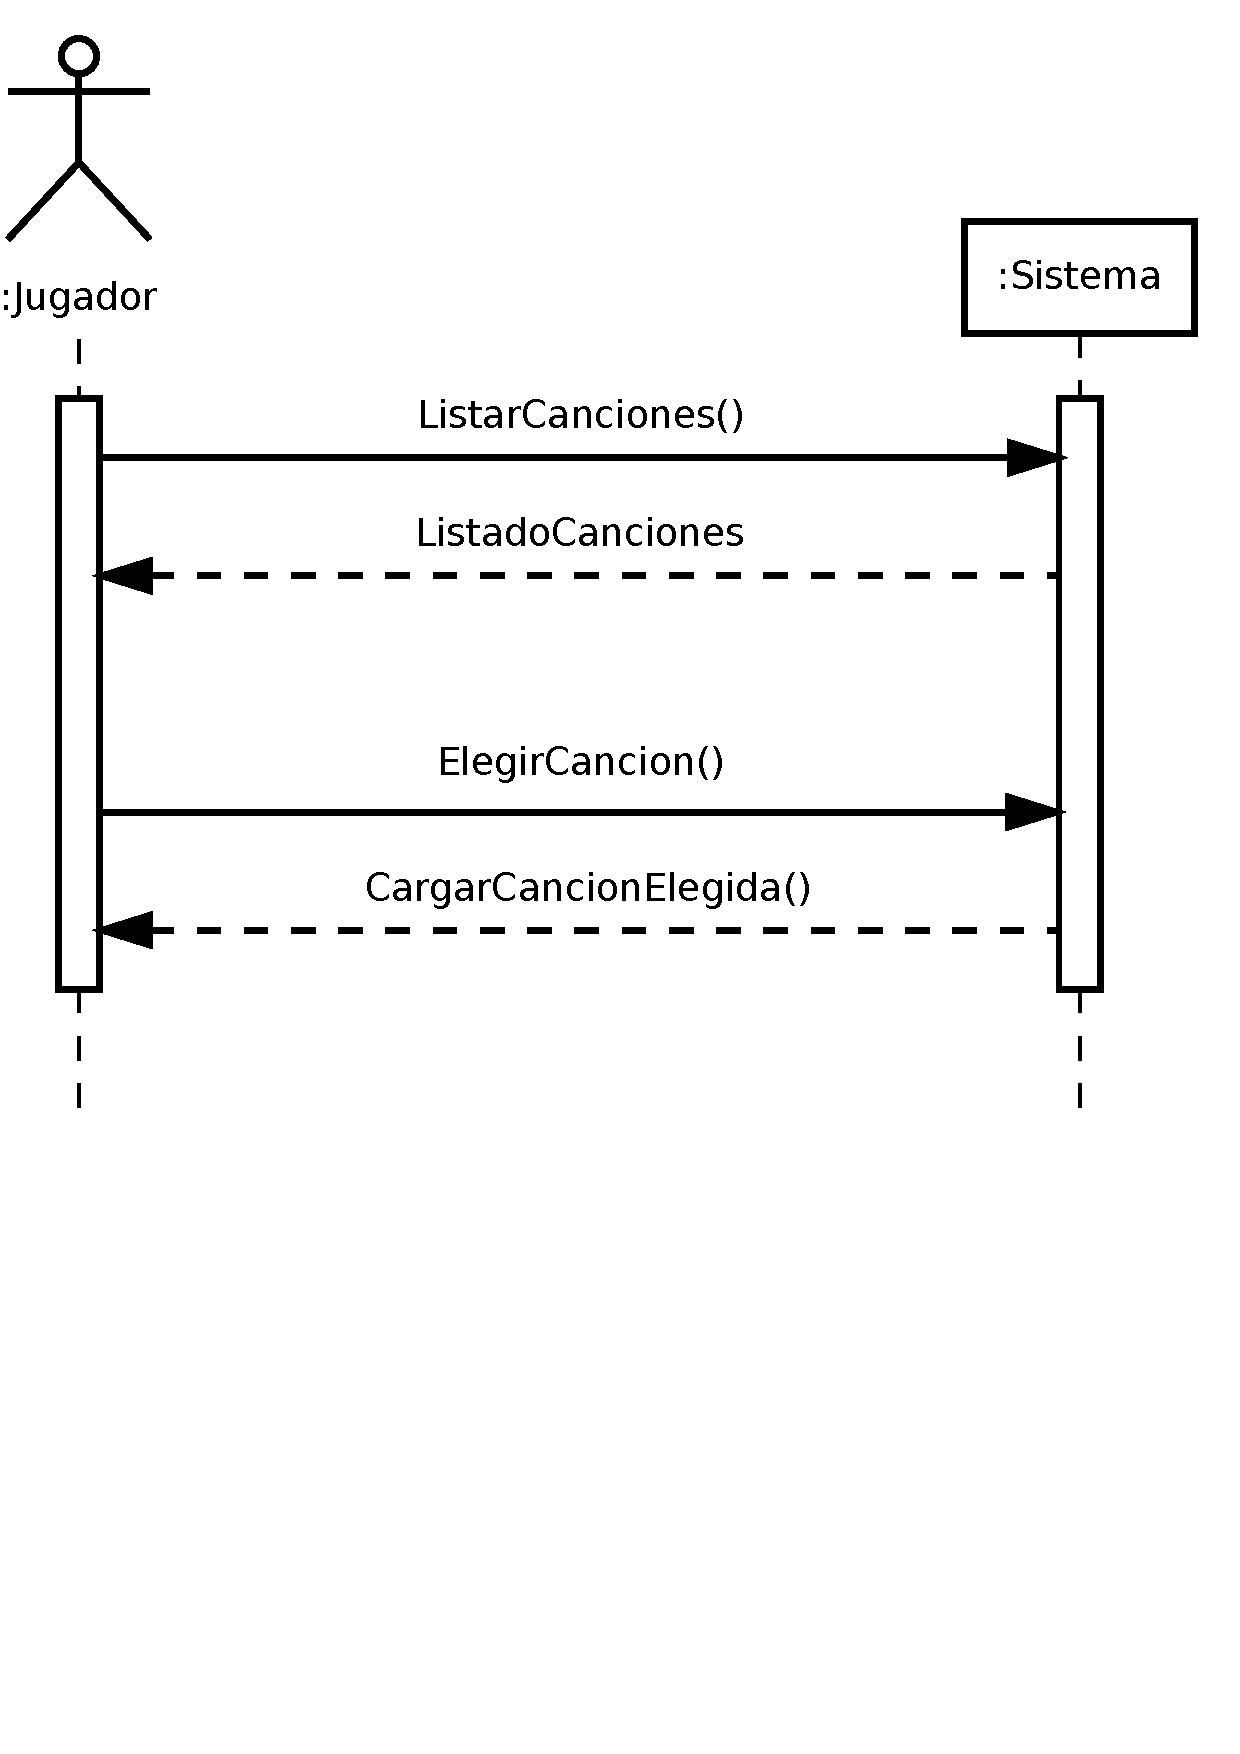
\includegraphics[trim=0cm 12cm 0cm 0cm, clip=true, width=0.5\textwidth]{4_analisis/diagsec_caso2_esc1}
  \caption{Diagrama de secuencia, selección de canción, escenario principal}
\end{figure}

\begin{description}
\item[Operación] ListarCanciones()
\item[Actores] \jugador\, \sistema\
\item[Responsabilidades] Cargar y mostrar la lista de canciones cargadas en el
  sistema.
\item[Precondiciones] Se ordenó la carga del estado \textit{EstadoMenuCanción}
\item[Postcondiciones] $\quad$
  \begin{itemize}
  \item El estado actual es una instancia de \textit{EstadoMenuCanción}.
  \item Se ha cargado la lista de canciones y se muestra en pantalla.
  \end{itemize}
\end{description}

\begin{description}
\item[Operación] ElegirCanción()
\item[Actores] \jugador\, \sistema\
\item[Responsabilidades] Cargar la canción que el usuario ha elegido para
  interpretar.
\item[Precondiciones] Existe una lista de canciones cargada de entre las que el
  usuario ha elegido una.
\item[Postcondiciones] $\quad$
  \begin{itemize}
  \item Se carga la canción indicada.
  \item Se oculta la lista de canciones.
  \item Se pasa a un sub-estado de interpretación de canción.
  \end{itemize}
\end{description}
\subsubsection{Escenario alternativo 3a}
\begin{figure}[h!]
  \centering
  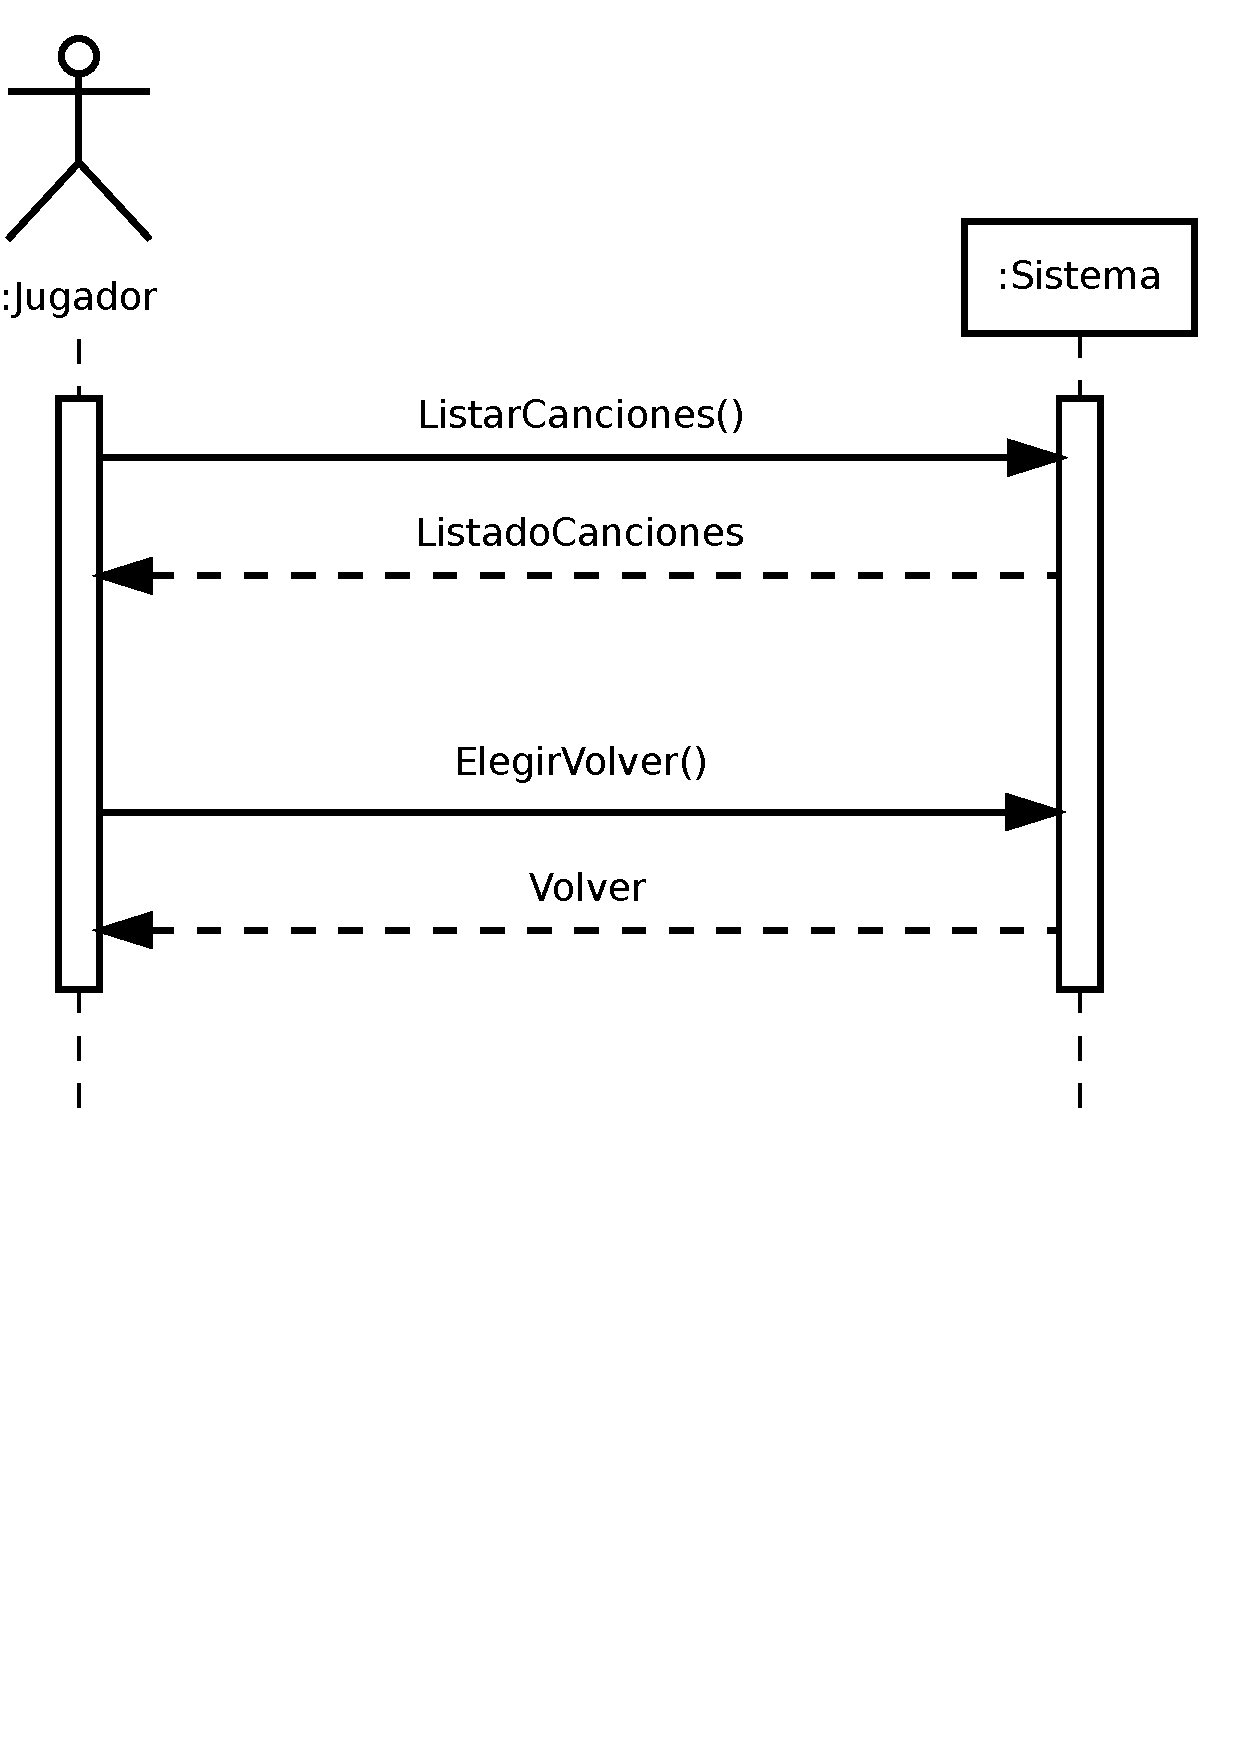
\includegraphics[trim=0cm 12cm 0cm 0cm, clip=true, width=0.5\textwidth]{4_analisis/diagsec_caso2_esc2}
  \caption{Diagrama de secuencia, selección de canción, escenario alternativo 3a}
\end{figure}
\begin{description}
\item[Operación] ElegirVolver()
\item[Actores] \jugador\, \sistema\
\item[Responsabilidades] Descargar la sección actual y volver al menú anterior.
\item[Precondiciones] El estado actual es una instancia de \textit{EstadoMenuCanción}.
\item[Postcondiciones] $\quad$
  \begin{itemize}
  \item El estado instancia de \textit{EstadoMenuCanción} queda descargado.
  \item Se carga y se muestra \textit{EstadoMenú}.
  \end{itemize}
\end{description}

\subsection{Interpretación de canción}
\begin{nota}
  No se reflejan los escenarios alternativos al estar englobados en la operación
  \textit{InteractuarConFlauta}.
\end{nota}

\subsubsection{Escenario principal}
\begin{figure}[h!]
  \centering
  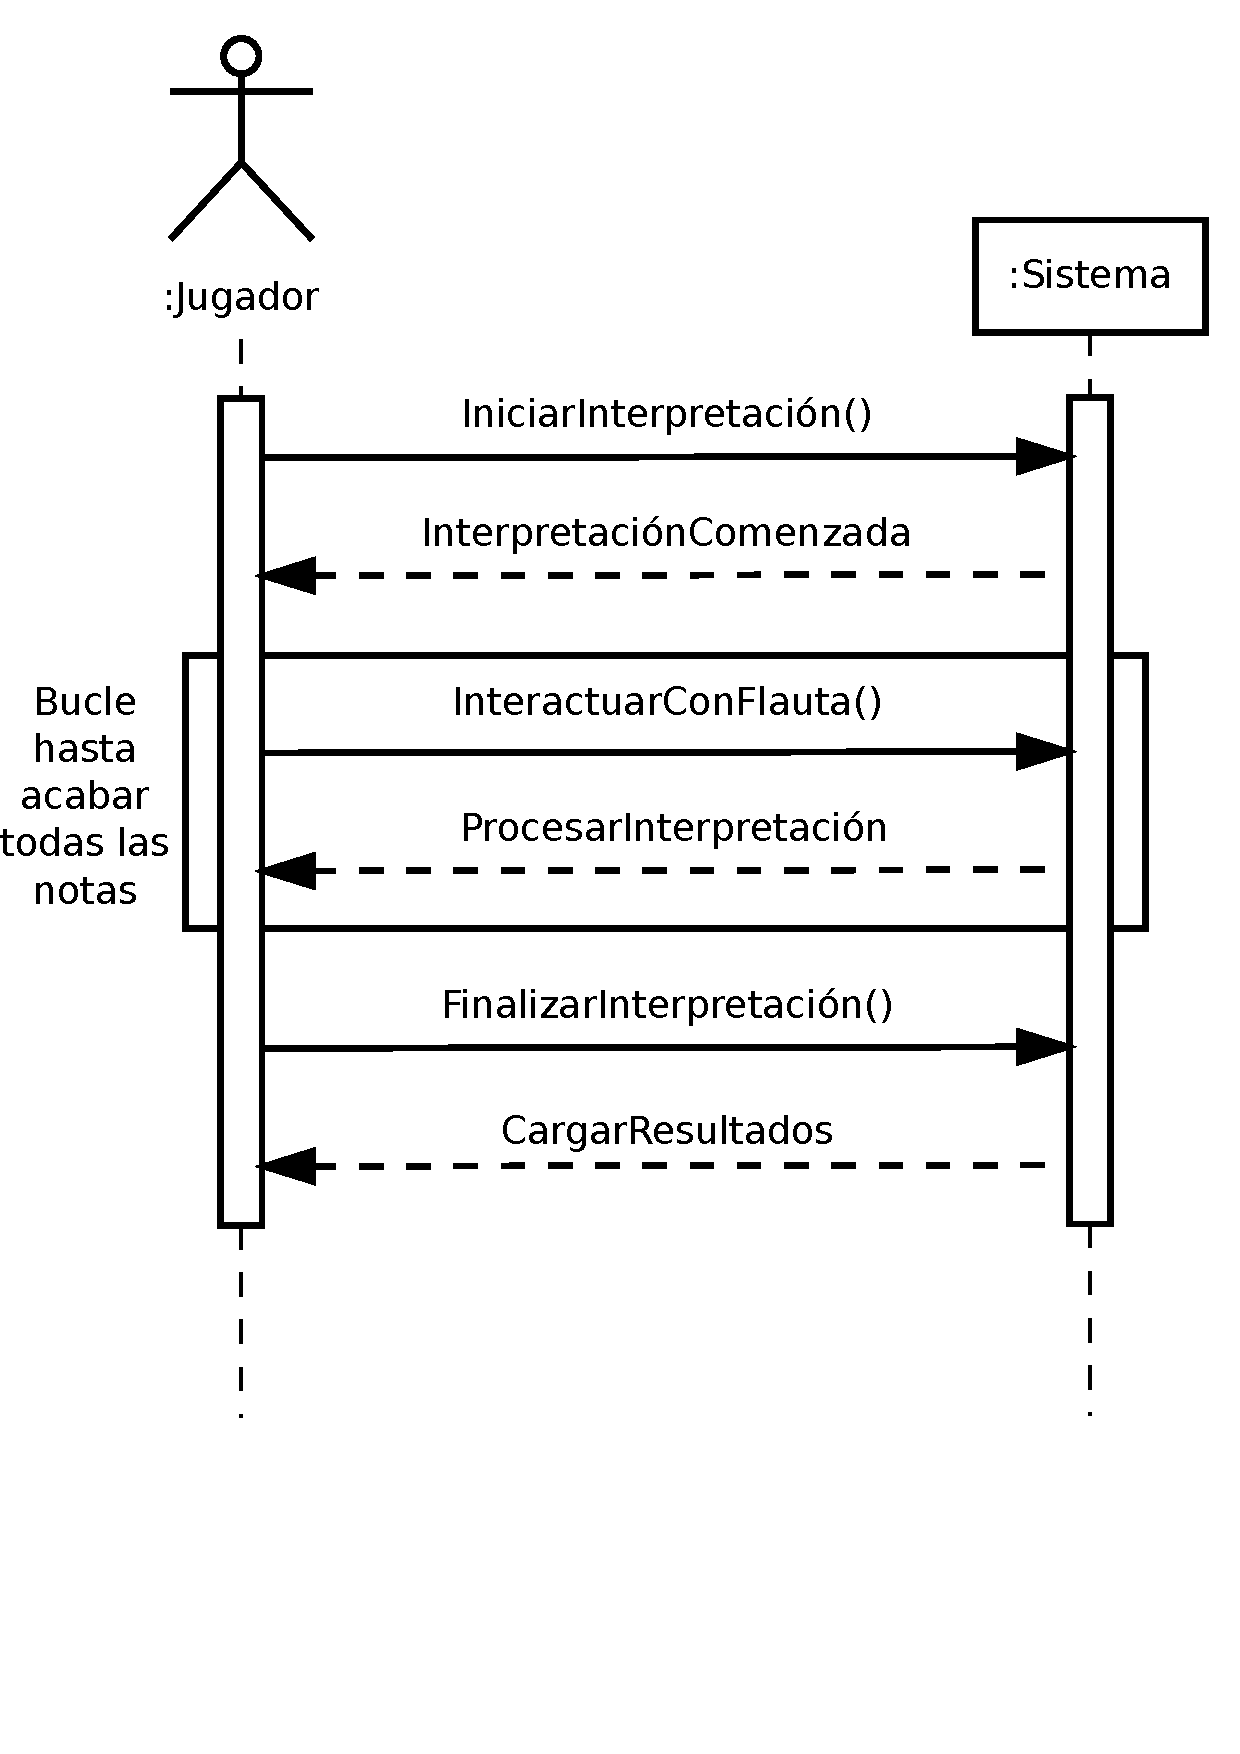
\includegraphics[trim=0cm 8cm 0cm 0cm, clip=true, width=0.5\textwidth]{4_analisis/diagsec_caso3}
  \caption{Diagrama de secuencia, interpretación de canción, escenario principal}
\end{figure}

\begin{description}
\item[Operación] IniciarInterpretación()
\item[Actores] \jugador\, \sistema\
\item[Responsabilidades] Parsear el fichero de canción, cargar la interfaz y
  comenzar la interpretación.
\item[Precondiciones] El usuario ha elegido una canción en el estado anterior.
\item[Postcondiciones] $\quad$
  \begin{itemize}
  \item Se muestra la interfaz de interpretación de canción.
  \item El fichero de canción queda cargado e interpretado, instanciando los
    elementos de la clase \textit{Nota} que sean necesarios.
  \item Comienza la interpretación
  \end{itemize}
\end{description}

\begin{description}
\item[Operación] InteractuarConFlauta()
\item[Actores] \jugador\, \sistema\
\item[Responsabilidades] El \jugador\ interactúa con el sistema mediante la
  flauta a través del micrófono, y el \sistema\ analiza los datos y muestra una
  respuesta en pantalla.
\item[Precondiciones] $\quad$
  \begin{itemize}
  \item La interpretación ha comenzado.
  \item El micrófono está correctamente configurado.
  \end{itemize}
\item[Postcondiciones] $\quad$
  \begin{itemize}
  \item El sistema captura y analiza los datos de audio.
  \item Según el análisis, el sistema responde de una forma u otra (según los
    escenarios alternativos 3a, 4a y 5a del caso de uso \textit{interpretación
      de canción}).
  \end{itemize}
\end{description}

\begin{description}
\item[Operación] FinalizarInterpretación()
\item[Actores] \jugador\, \sistema\
\item[Responsabilidades] Descargar la pantalla de interpretación, descargar la
  canción y finalizar la interpretación.
\item[Precondiciones] Todas las notas se han interpretado.
\item[Postcondiciones] $\quad$
  \begin{itemize}
  \item Se descarga la \textit{Canción} actual.
  \item Se ocultan los elementos de la interfaz de interpretación.
  \item Se lanza la sección de puntuación.
  \end{itemize}
\end{description}


\subsection{Resultados de interpretación}

\subsubsection{Escenario principal}
\begin{figure}[h!]
  \centering
  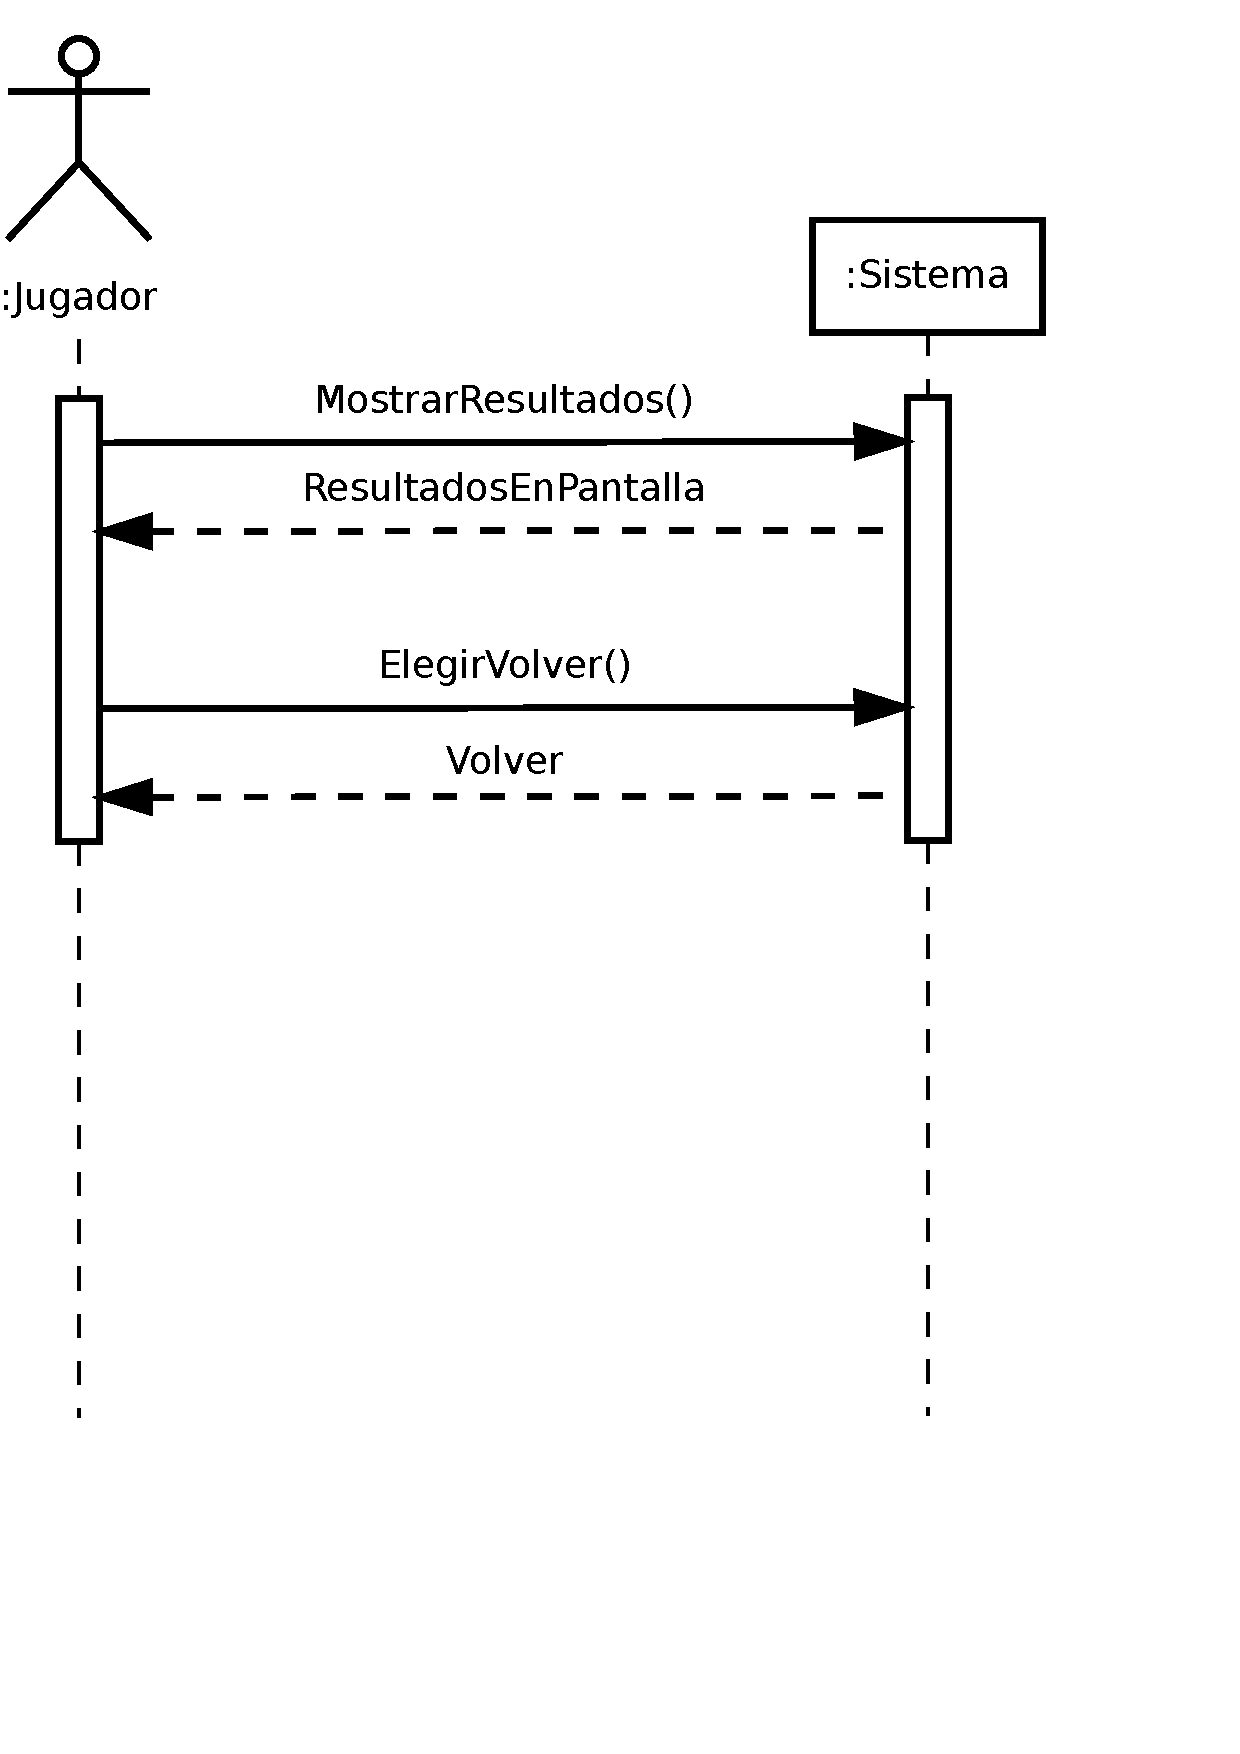
\includegraphics[trim=0cm 12cm 0cm 0cm, clip=true, width=0.5\textwidth]{4_analisis/diagsec_caso4}
  \caption{Diagrama de secuencia, resultados de interpretación, escenario principal}
\end{figure}

\begin{description}
\item[Operación] MostrarResultados()
\item[Actores] \jugador\, \sistema\
\item[Responsabilidades] Interpretar los resultados de la interpretación y
  mostrar los resultados en pantalla.
\item[Precondiciones] El \jugador\ ha concluído satisfactoriamente una
  interpretación completa de una canción, obteniendo una suma de puntos $X$.
\item[Postcondiciones] Mostrar en pantalla los resultados en forma de porcentaje
  de aciertos, y un mensaje según aquél.
\end{description}

\begin{description}
\item[Operación] ElegirVolver()
\item[Actores] \jugador\, \sistema\
\item[Responsabilidades] Descargar la sección actual y volver al menú anterior.
\item[Precondiciones] $\quad$
  \begin{itemize}
  \item La aplicación se encuentra en la pantalla de muestra de resultados.
  \item El usuario ha pulsado la tecla \texttt{escape} o el botón \textit{volver}.
  \end{itemize}
\item[Postcondiciones] $\quad$
  \begin{itemize}
  \item Se descargan todos los datos referentes a la canción actual.
  \item Se carga y se muestra \textit{EstadoMenúCanciones}.
  \end{itemize}
\end{description}

\subsection{Analizador de notas}

\begin{nota}
  No se reflejan los escenarios alternativos al estar englobados en la operación
  \textit{InteractuarConFlauta}.
\end{nota}

\subsubsection{Escenario principal}
\begin{figure}[h!]
  \centering
  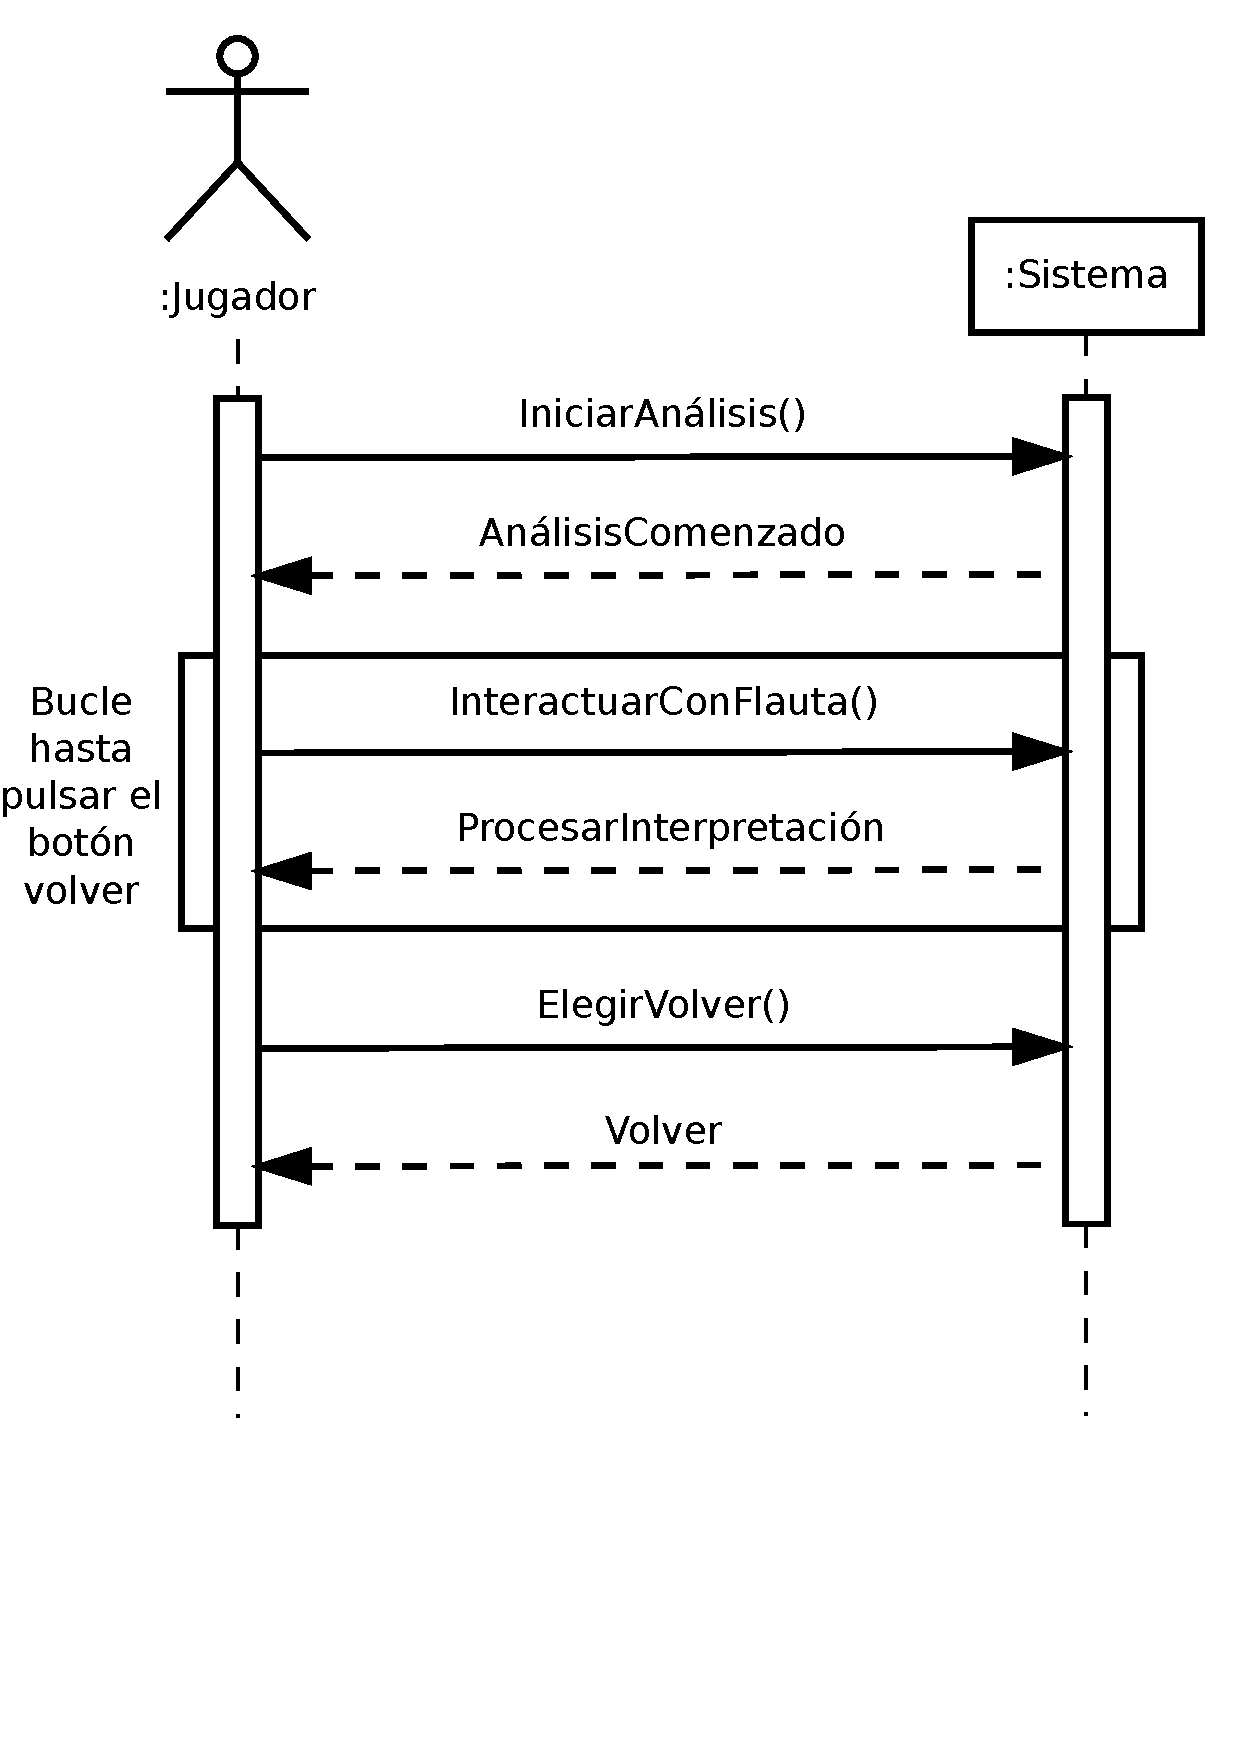
\includegraphics[trim=0cm 8cm 0cm 0cm, clip=true, width=0.5\textwidth]{4_analisis/diagsec_caso5}
  \caption{Diagrama de secuencia, interpretación de canción, escenario principal}
\end{figure}

\begin{description}
\item[Operación] IniciarAnálisis
\item[Actores] \jugador\, \sistema\
\item[Responsabilidades] Cargar la interfaz e iniciar el análisis de notas.
\item[Precondiciones] El usuario eligió la sección \textit{Analizador de notas}
  en el menú principal.
\item[Postcondiciones] $\quad$
  \begin{itemize}
  \item Aparece la interfaz del analizador de notas.
  \item Se inicia el análisis de notas
  \end{itemize}
\end{description}

\begin{description}
\item[Operación] InteractuarConFlauta
\item[Actores] \jugador\, \sistema\
\item[Responsabilidades] El \jugador\ toca notas en la flauta y el \sistema\
  captura y reconoce el audio, indicando la nota tocada en pantalla.

\item[Precondiciones] Se ha iniciado el análisis.

\item[Postcondiciones] $\quad$
  \begin{itemize}
  \item El \sistema\ recoge y analiza el sonido que emite la flauta del \jugador.
  \item El \sistema\ representa en pantalla la nota identificada, o no muestra
    nada en caso de identificación defectuosa.
  \end{itemize}
\end{description}

% \begin{description}
% \item[Operación] ElegirVolver()
% \item[Actores] \jugador\, \sistema\
% \item[Responsabilidades] Descargar la sección actual y volver al menú anterior.
% \item[Precondiciones] $\quad$
%   \begin{itemize}
%   \item El estado actual es una instancia de \textit{EstadoAnalizador}.
%   \item Hay un análisis en curso.  
%   \end{itemize}
  
% \item[Postcondiciones] $\quad$
%   \begin{itemize}
%   \item Concluye el análisis actual.
%   \item Se destruye el estado.
%   \item Se carga y se muestra \textit{EstadoMenú}.
%   \end{itemize}
% \end{description}

\subsection{Calibración de micrófono}

\subsubsection{Escenario principal}
\begin{figure}[h!]
  \centering
  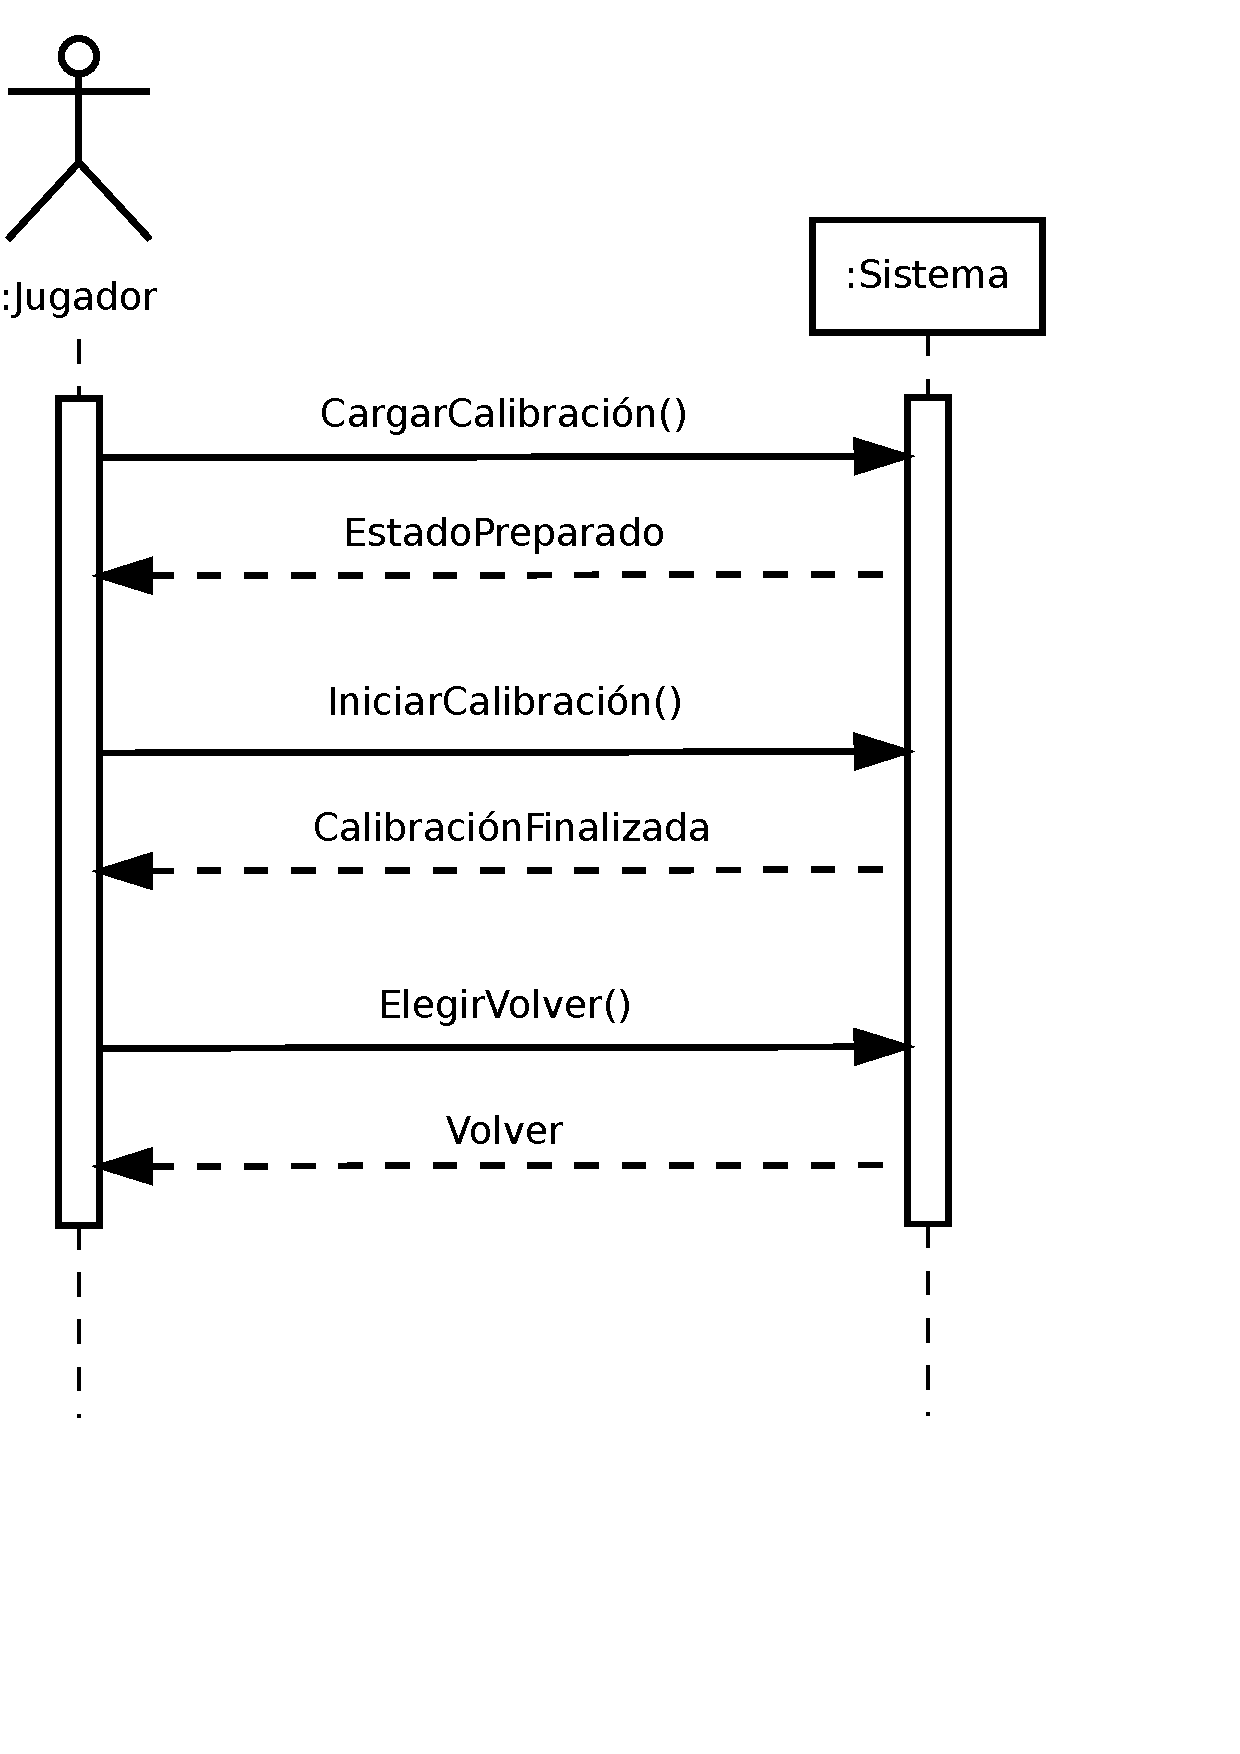
\includegraphics[trim=0cm 8cm 0cm 0cm, clip=true, width=0.5\textwidth]{4_analisis/diagsec_caso6_esc1}
  \caption{Diagrama de secuencia, calibración de micrófono, escenario principal}
\end{figure}

\begin{description}
\item[Operación] CargarCalibración()
\item[Actores] \jugador\, \sistema\
\item[Responsabilidades] Cargar la sección y preparar el sistema para comenzar
  la calibración del micrófono.
\item[Precondiciones] El usuario ha elegido en el menú principal la opción
  \textit{Calibrar micrófono}.
\item[Postcondiciones] La sección está cargada y la calibración lista para
  iniciarse.
\end{description}

\begin{description}
\item[Operación] CalibrarMicrófono()
\item[Actores] \jugador\, \sistema\
\item[Responsabilidades] Llevar a cabo la calibración correcta del micrófono.
\item[Precondiciones] El usuario ha lanzado la calibración del micrófono.
\item[Postcondiciones] $\quad$
  \begin{itemize}
  \item Se cierra el sistema de sonido.
  \item Se obtiene un valor umbral de ruido ambiente, fruto de una calibración
    exitosa.
  \end{itemize}
\end{description}

\begin{description}
\item[Operación] ElegirVolver()
\item[Actores] \jugador\, \sistema\
\item[Responsabilidades] Descargar la sección actual y volver al menú anterior.
\item[Precondiciones] $\quad$
  \begin{itemize}
  \item La calibración ha concluído exitosamente.
  \item El usuario ha pulsado la tecla \texttt{escape} o el botón \textit{volver}.
  \end{itemize}
\item[Postcondiciones] $\quad$
  \begin{itemize}
  \item Se descarga la sección actual.
  \item Se carga y se muestra \textit{EstadoMenúCanciones}.
  \end{itemize}
\end{description}

\subsubsection{Escenario alternativo 5a}
\begin{figure}[h!]
  \centering
  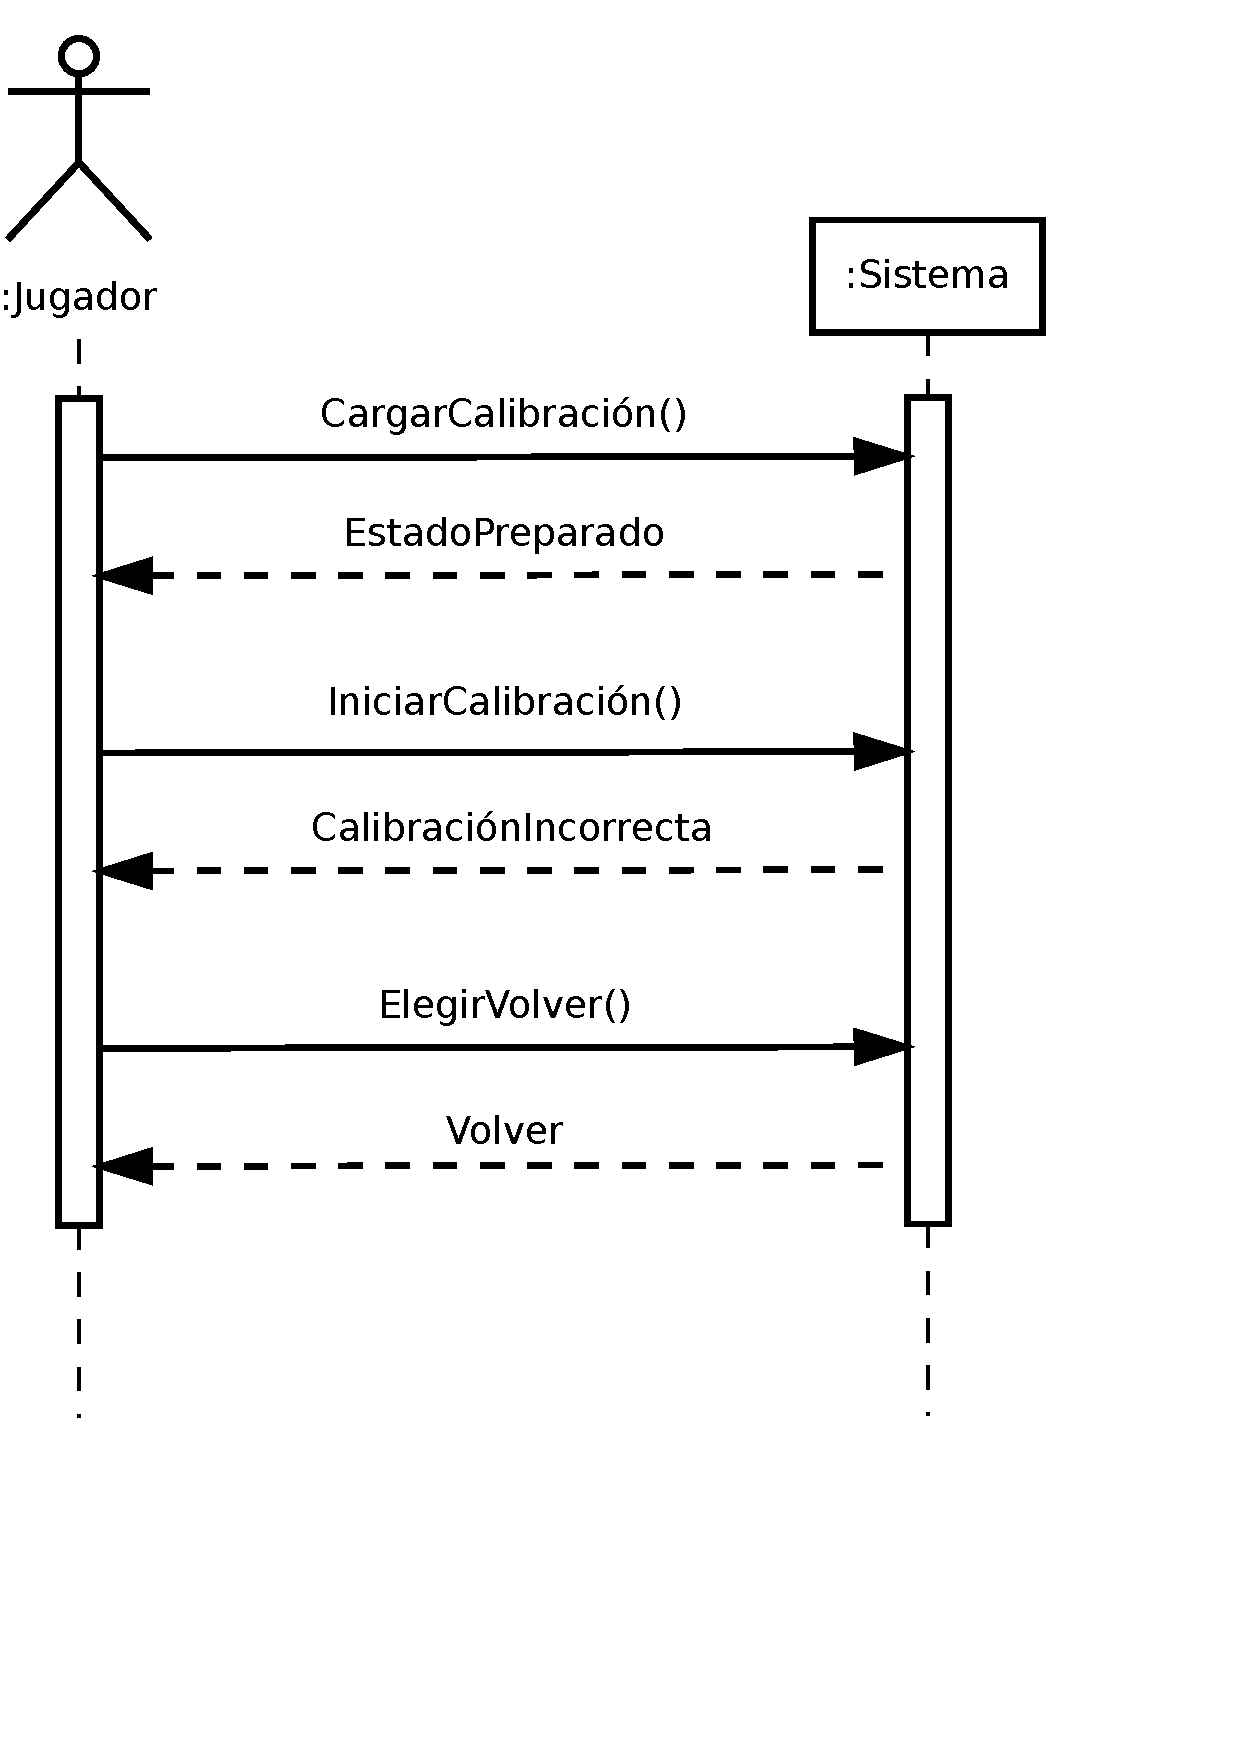
\includegraphics[trim=0cm 8cm 0cm 0cm, clip=true, width=0.5\textwidth]{4_analisis/diagsec_caso6_esc2}
  \caption{Diagrama de secuencia, calibración de micrófono, escenario principal}
\end{figure}
\begin{description}
\item[Operación] CalibrarMicrófono()
\item[Actores] \jugador\, \sistema\
\item[Responsabilidades] Llevar a cabo la calibración correcta del micrófono.
\item[Precondiciones] El usuario ha lanzado la calibración del micrófono.
\item[Postcondiciones] $\quad$
  \begin{itemize}
  \item Se cierra el sistema de sonido.
  \item La calibración ha fallado.
  \item No se obtiene valor umbral de ruido ambiental.
  \end{itemize}
\end{description}

\subsection{Selección de lecciones}

\subsubsection{Escenario principal}
\begin{figure}[h!]
  \centering
  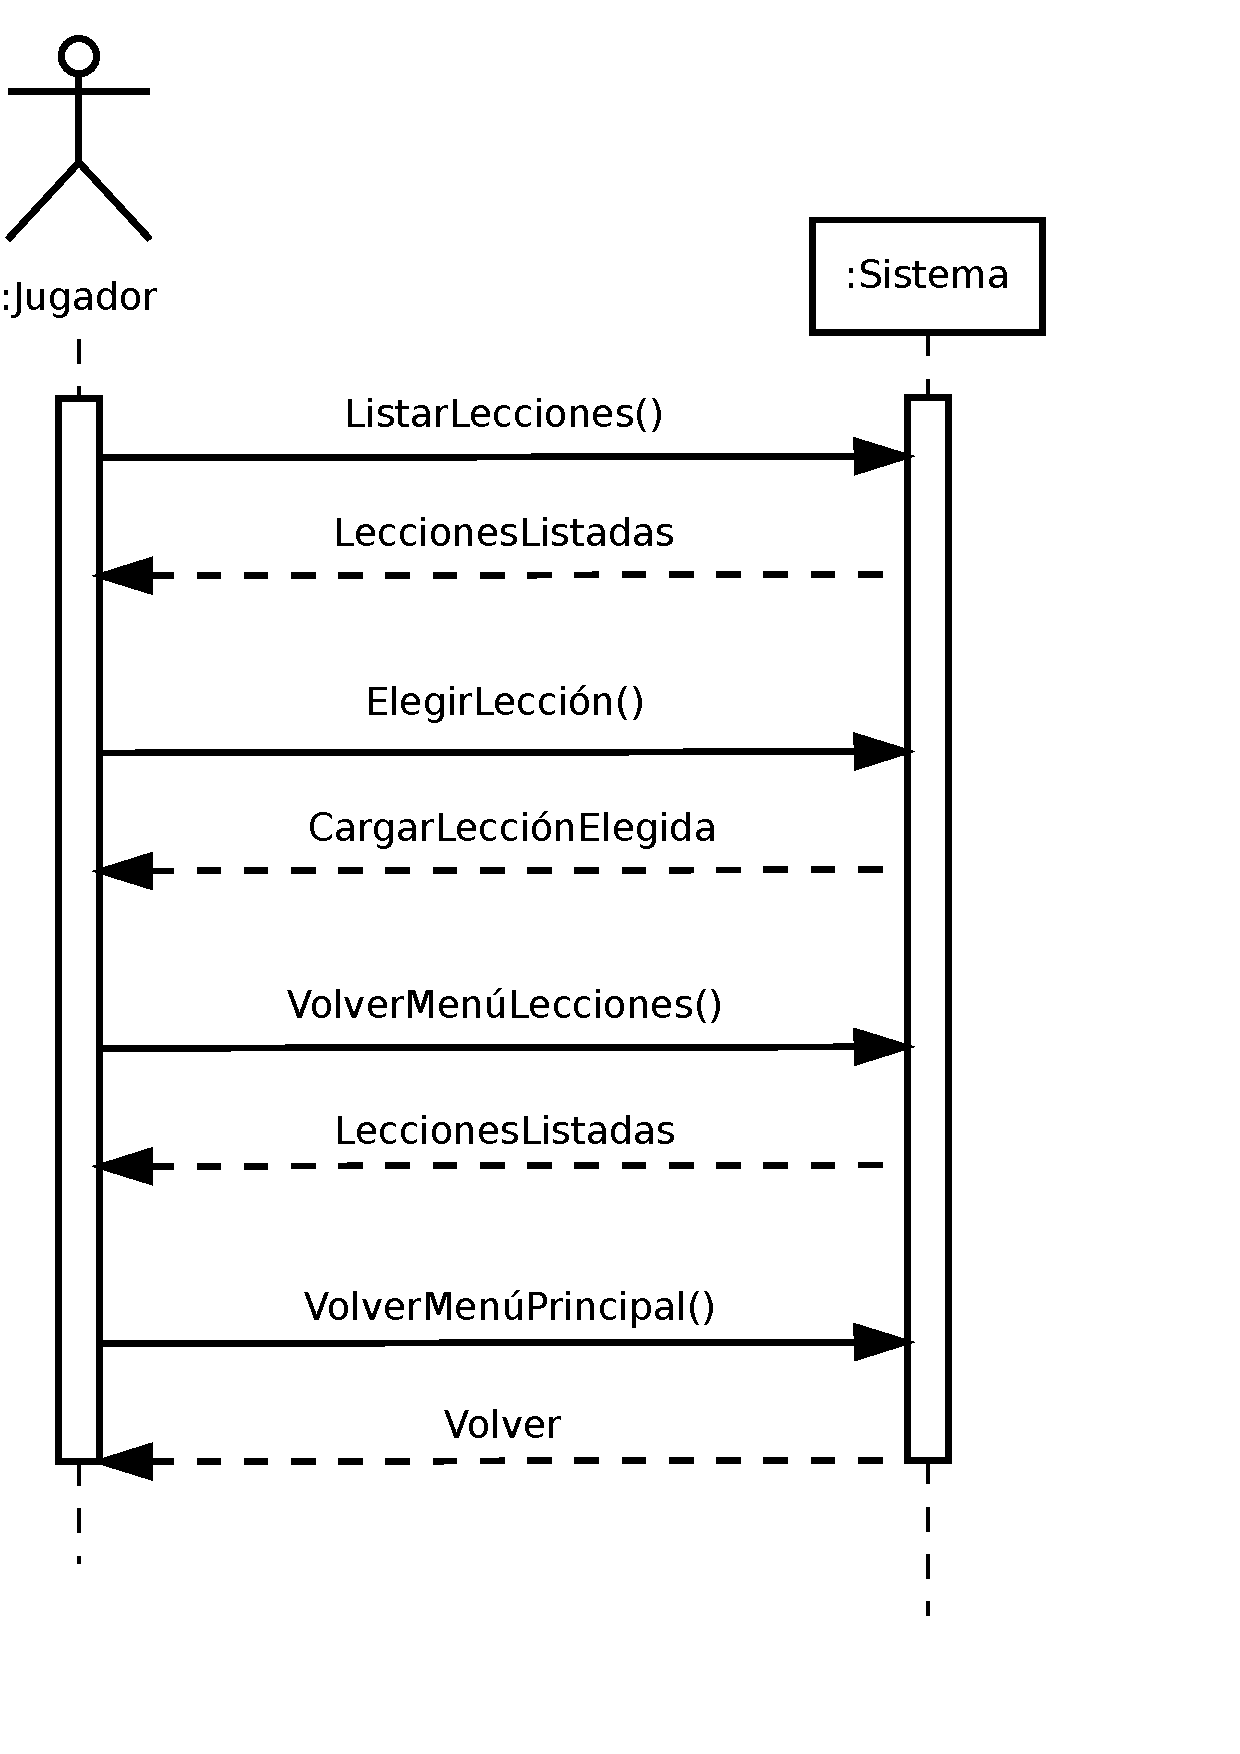
\includegraphics[trim=0cm 4cm 0cm 0cm, clip=true, width=0.5\textwidth]{4_analisis/diagsec_caso7_esc1}
  \caption{Diagrama de secuencia, selección delecciones, escenario principal}
\end{figure}


\begin{description}
\item[Operación] ListarLecciones()
\item[Actores] \jugador\, \sistema\
\item[Responsabilidades] Mostrar el menú de selección de lecciones y listar
  todas las lecciones disponibles.
\item[Precondiciones] El usuario eligió la opción \textit{Lecciones} en el menú
  principal.
\item[Postcondiciones] $\quad$
  \begin{itemize}
  \item Se muestra la interfaz del menú de selección de lecciones.
  \item Se listan las lecciones cargadas en el sistema
  \end{itemize}
\end{description}

\begin{description}
\item[Operación] ElegirLección()
\item[Actores] \jugador\, \sistema\
\item[Responsabilidades] Cargar y mostrar la lección elegida por el usuario.
\item[Precondiciones] El menú de selección de lecciones está cargado y el
  usuario ha elegido una de las lecciones.
\item[Postcondiciones]$\quad$
  \begin{itemize}
  \item Se oculta el menú de selección de lecciones.
  \item Se interpreta el fichero de lección elegido.
  \item Se muestran los elementos multimedia pertenecientes a la lección
    elegida.
  \end{itemize}
\end{description}

\begin{description}
\item[Operación] VolverMenuLecciones()
\item[Actores] \jugador\, \sistema\
\item[Responsabilidades] Descargar la lección actual y volver al menú anterior.
\item[Precondiciones] $\quad$
  \begin{itemize}
  \item El usuario ha terminado de ver la lección elegida.
  \item El usuario ha pulsado la tecla \texttt{escape} o el botón \textit{volver}.
  \end{itemize}
\item[Postcondiciones] $\quad$
  \begin{itemize}
  \item Se descarga la lección actual.
  \item Se muestra de nuevo el menú de selección de lecciones.
  \end{itemize}
\end{description}

\begin{description}
\item[Operación] VolverMenuPrincipal()
\item[Actores] \jugador\, \sistema\
\item[Responsabilidades] Descargar el menú de selección de lecciones y volver al
  menú principal.
\item[Precondiciones] El usuario ha pulsado la tecla \texttt{escape} o el botón \textit{volver}.
\item[Postcondiciones] $\quad$
  \begin{itemize}
  \item Se descarga el menú de selección de lecciones.
  \item Se carga y muestra el menú principal
  \end{itemize}
\end{description}

\subsubsection{Escenario alternativo}
\begin{figure}[h!]
  \centering
  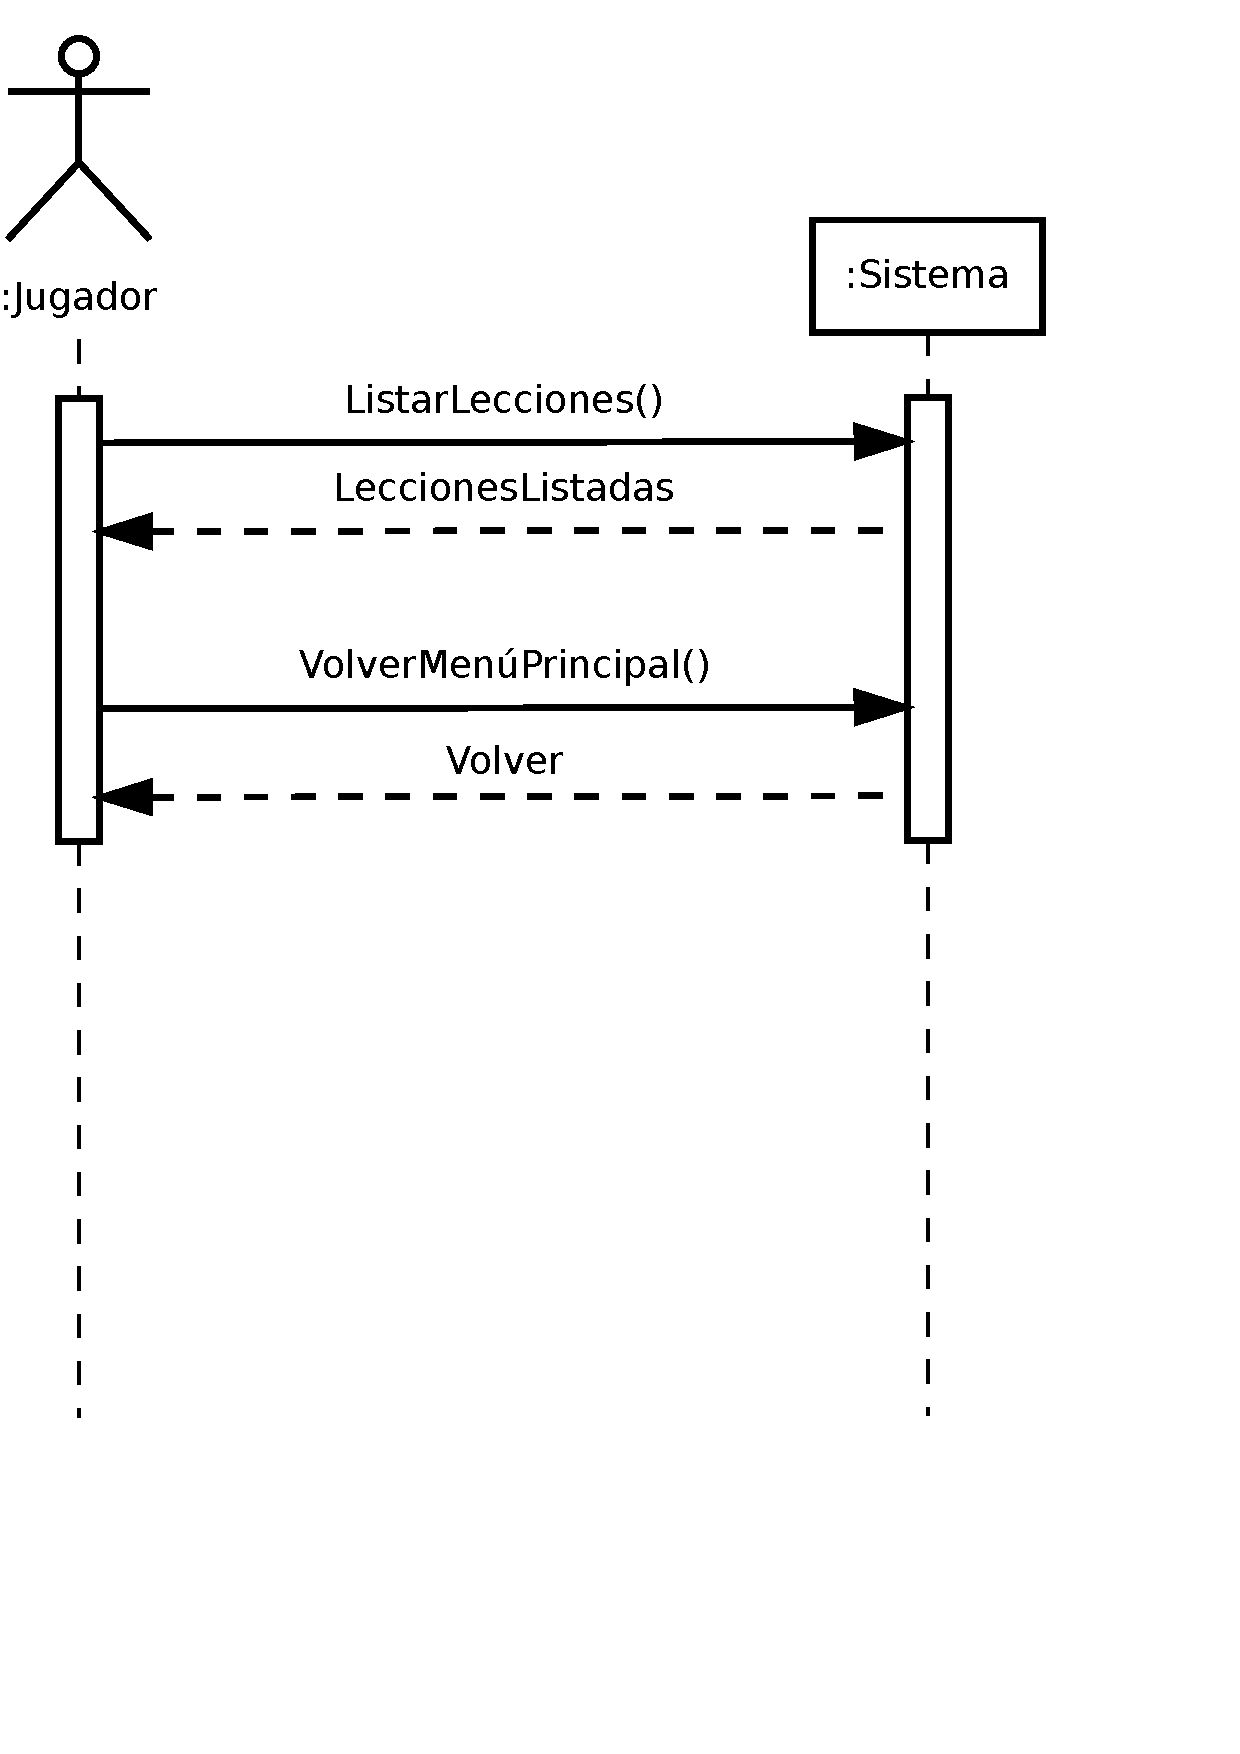
\includegraphics[trim=0cm 12cm 0cm 0cm, clip=true, width=0.5\textwidth]{4_analisis/diagsec_caso7_esc2}
  \caption{Diagrama de secuencia, selección de lecciones, escenario alternativo}
\end{figure}

\begin{description}
\item[Operación] ListarLecciones()
\item[Actores] \jugador\, \sistema\
\item[Responsabilidades] Mostrar el menú de selección de lecciones y listar
  todas las lecciones disponibles.
\item[Precondiciones] El usuario eligió la opción \textit{Lecciones} en el menú
  principal.
\item[Postcondiciones] $\quad$
  \begin{itemize}
  \item Se muestra la interfaz del menú de selección de lecciones.
  \item Se listan las lecciones cargadas en el sistema
  \end{itemize}
\end{description}

\begin{description}
\item[Operación] VolverMenuPrincipal()
\item[Actores] \jugador\, \sistema\
\item[Responsabilidades] Descargar el menú de selección de lecciones y volver al
  menú principal.
\item[Precondiciones] El usuario ha pulsado la tecla \texttt{escape} o el botón \textit{volver}.
\item[Postcondiciones] $\quad$
  \begin{itemize}
  \item Se descarga el menú de selección de lecciones.
  \item Se carga y muestra el menú principal
  \end{itemize}
\end{description}

%%% Local Variables: 
%%% mode: latex
%%% TeX-master: "../memoria"
%%% End: 